\PassOptionsToPackage{unicode=true}{hyperref} % options for packages loaded elsewhere
\PassOptionsToPackage{hyphens}{url}
%
\documentclass[a4paperpaper,openright]{book}
\usepackage{lmodern}
\usepackage{amssymb,amsmath}
\usepackage{ifxetex,ifluatex}
\usepackage{fixltx2e} % provides \textsubscript
\ifnum 0\ifxetex 1\fi\ifluatex 1\fi=0 % if pdftex
  \usepackage[T1]{fontenc}
  \usepackage[utf8]{inputenc}
  \usepackage{textcomp} % provides euro and other symbols
\else % if luatex or xelatex
  \usepackage{unicode-math}
  \defaultfontfeatures{Ligatures=TeX,Scale=MatchLowercase}
\fi
% use upquote if available, for straight quotes in verbatim environments
\IfFileExists{upquote.sty}{\usepackage{upquote}}{}
% use microtype if available
\IfFileExists{microtype.sty}{%
\usepackage[]{microtype}
\UseMicrotypeSet[protrusion]{basicmath} % disable protrusion for tt fonts
}{}
\IfFileExists{parskip.sty}{%
\usepackage{parskip}
}{% else
\setlength{\parindent}{0pt}
\setlength{\parskip}{6pt plus 2pt minus 1pt}
}
\usepackage{hyperref}
\hypersetup{
            pdfborder={0 0 0},
            breaklinks=true}
\urlstyle{same}  % don't use monospace font for urls
\usepackage{color}
\usepackage{fancyvrb}
\newcommand{\VerbBar}{|}
\newcommand{\VERB}{\Verb[commandchars=\\\{\}]}
\DefineVerbatimEnvironment{Highlighting}{Verbatim}{commandchars=\\\{\}}
% Add ',fontsize=\small' for more characters per line
\newenvironment{Shaded}{}{}
\newcommand{\AlertTok}[1]{\textcolor[rgb]{1.00,0.00,0.00}{\textbf{#1}}}
\newcommand{\AnnotationTok}[1]{\textcolor[rgb]{0.38,0.63,0.69}{\textbf{\textit{#1}}}}
\newcommand{\AttributeTok}[1]{\textcolor[rgb]{0.49,0.56,0.16}{#1}}
\newcommand{\BaseNTok}[1]{\textcolor[rgb]{0.25,0.63,0.44}{#1}}
\newcommand{\BuiltInTok}[1]{#1}
\newcommand{\CharTok}[1]{\textcolor[rgb]{0.25,0.44,0.63}{#1}}
\newcommand{\CommentTok}[1]{\textcolor[rgb]{0.38,0.63,0.69}{\textit{#1}}}
\newcommand{\CommentVarTok}[1]{\textcolor[rgb]{0.38,0.63,0.69}{\textbf{\textit{#1}}}}
\newcommand{\ConstantTok}[1]{\textcolor[rgb]{0.53,0.00,0.00}{#1}}
\newcommand{\ControlFlowTok}[1]{\textcolor[rgb]{0.00,0.44,0.13}{\textbf{#1}}}
\newcommand{\DataTypeTok}[1]{\textcolor[rgb]{0.56,0.13,0.00}{#1}}
\newcommand{\DecValTok}[1]{\textcolor[rgb]{0.25,0.63,0.44}{#1}}
\newcommand{\DocumentationTok}[1]{\textcolor[rgb]{0.73,0.13,0.13}{\textit{#1}}}
\newcommand{\ErrorTok}[1]{\textcolor[rgb]{1.00,0.00,0.00}{\textbf{#1}}}
\newcommand{\ExtensionTok}[1]{#1}
\newcommand{\FloatTok}[1]{\textcolor[rgb]{0.25,0.63,0.44}{#1}}
\newcommand{\FunctionTok}[1]{\textcolor[rgb]{0.02,0.16,0.49}{#1}}
\newcommand{\ImportTok}[1]{#1}
\newcommand{\InformationTok}[1]{\textcolor[rgb]{0.38,0.63,0.69}{\textbf{\textit{#1}}}}
\newcommand{\KeywordTok}[1]{\textcolor[rgb]{0.00,0.44,0.13}{\textbf{#1}}}
\newcommand{\NormalTok}[1]{#1}
\newcommand{\OperatorTok}[1]{\textcolor[rgb]{0.40,0.40,0.40}{#1}}
\newcommand{\OtherTok}[1]{\textcolor[rgb]{0.00,0.44,0.13}{#1}}
\newcommand{\PreprocessorTok}[1]{\textcolor[rgb]{0.74,0.48,0.00}{#1}}
\newcommand{\RegionMarkerTok}[1]{#1}
\newcommand{\SpecialCharTok}[1]{\textcolor[rgb]{0.25,0.44,0.63}{#1}}
\newcommand{\SpecialStringTok}[1]{\textcolor[rgb]{0.73,0.40,0.53}{#1}}
\newcommand{\StringTok}[1]{\textcolor[rgb]{0.25,0.44,0.63}{#1}}
\newcommand{\VariableTok}[1]{\textcolor[rgb]{0.10,0.09,0.49}{#1}}
\newcommand{\VerbatimStringTok}[1]{\textcolor[rgb]{0.25,0.44,0.63}{#1}}
\newcommand{\WarningTok}[1]{\textcolor[rgb]{0.38,0.63,0.69}{\textbf{\textit{#1}}}}
\usepackage{graphicx,grffile}
\makeatletter
\def\maxwidth{\ifdim\Gin@nat@width>\linewidth\linewidth\else\Gin@nat@width\fi}
\def\maxheight{\ifdim\Gin@nat@height>\textheight\textheight\else\Gin@nat@height\fi}
\makeatother
% Scale images if necessary, so that they will not overflow the page
% margins by default, and it is still possible to overwrite the defaults
% using explicit options in \includegraphics[width, height, ...]{}
\setkeys{Gin}{width=\maxwidth,height=\maxheight,keepaspectratio}
\setlength{\emergencystretch}{3em}  % prevent overfull lines
\providecommand{\tightlist}{%
  \setlength{\itemsep}{0pt}\setlength{\parskip}{0pt}}
\setcounter{secnumdepth}{0}
% Redefines (sub)paragraphs to behave more like sections
\ifx\paragraph\undefined\else
\let\oldparagraph\paragraph
\renewcommand{\paragraph}[1]{\oldparagraph{#1}\mbox{}}
\fi
\ifx\subparagraph\undefined\else
\let\oldsubparagraph\subparagraph
\renewcommand{\subparagraph}[1]{\oldsubparagraph{#1}\mbox{}}
\fi

% set default figure placement to htbp
\makeatletter
\def\fps@figure{htbp}
\makeatother

% Table of contents formatting
\renewcommand{\contentsname}{Table of Contents}
\setcounter{tocdepth}{3}

\setcounter{secnumdepth}{4}


% \renewcommand\thesection{\Roman{section}}

 
% Headers and page numbering 
\usepackage{fancyhdr}

\fancyhead{}
\fancyhead[R]{\leftmark}
\renewcommand{\headrulewidth}{0.4pt}

\fancyfoot[R]{\thepage}
\fancyfoot[C]{}
\fancyfoot[L]{\textit{An Introduction to Symfony 6 \copyright Matt Smith 2022}}
\renewcommand{\footrulewidth}{0.4pt}

\pagestyle{fancy}

% Fonts and typesetting
\setsansfont{Verdana}

% Set figure legends and captions to be smaller sized sans serif font
\usepackage[font={footnotesize,sf}]{caption}

\usepackage{siunitx}

% Adjust spacing between lines to 1.5
\usepackage{setspace}
\onehalfspacing
\raggedbottom

% Set margins
\usepackage[top=1.25in,bottom=1.25in]{geometry}

% Chapter styling
\usepackage[grey]{quotchap}
\makeatletter
\renewcommand*{\chapnumfont}{%
  \usefont{T1}{\@defaultcnfont}{b}{n}\fontsize{80}{100}\selectfont% Default: 100/130
  \color{chaptergrey}%
}
\makeatother

% Set colour of links to black so that they don't show up when printed
\usepackage{hyperref}
\hypersetup{colorlinks=true, linkcolor=black}

% Tables
\usepackage{booktabs}
\usepackage{threeparttable}
\usepackage{array}
\newcolumntype{x}[1]{%
>{\centering\arraybackslash}m{#1}}%

% Allow for long captions and float captions on opposite page of figures 
\usepackage[rightFloats, CaptionBefore]{fltpage}

% Don't let floats cross subsections
\usepackage[section,subsection]{extraplaceins}

\date{}

\begin{document}

\hypertarget{symfony-example---lab-sheet-1}{%
\chapter{Symfony example - Lab Sheet
1}\label{symfony-example---lab-sheet-1}}

This lab sheet ensures:

\begin{enumerate}
\def\labelenumi{\arabic{enumi}.}
\item
  You have all software setup for the module on your computer
\item
  You have run and used the kinds of web applications you'll be creating
  in the module
\end{enumerate}

\begin{figure}
\centering
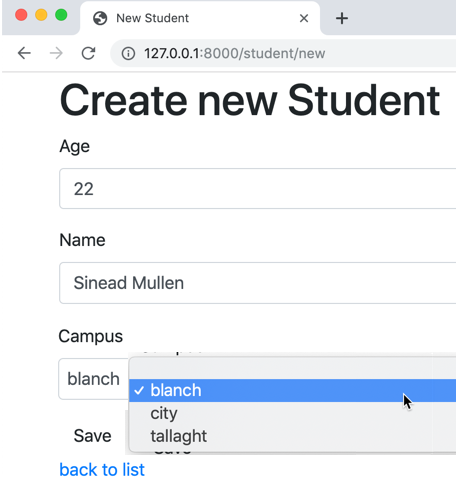
\includegraphics[width=0.5\textwidth,height=\textheight]{./tex2pdf.-2b0e1314f8bbbae5/06166ca531c57ddfbf4405cd4fecb47fcec83322.png}
\caption{Screenshot showing new Student form with Campus choice dropdown
menu}
\end{figure}

\hypertarget{preparation}{%
\section{Preparation}\label{preparation}}

\hypertarget{ensure-php-is-installed-on-your-computer}{%
\section{Ensure PHP is installed on your
computer}\label{ensure-php-is-installed-on-your-computer}}

You need PHP version 8.1.1 or later.

Open a command line terminal (e.g.~the \texttt{cmd} application in
Windows) and check your PHP version at the command line with:

\begin{Shaded}
\begin{Highlighting}[]
\NormalTok{    $ }\ExtensionTok{php}\NormalTok{ -v}
    \ExtensionTok{PHP}\NormalTok{ 8.1.1 (cli) }\KeywordTok{(}\ExtensionTok{built}\NormalTok{: Dec 15 2021 09:54:28}\KeywordTok{)} \KeywordTok{(}\ExtensionTok{NTS}\KeywordTok{)}
    \ExtensionTok{Copyright}\NormalTok{ (c) }\ExtensionTok{1997-2017}\NormalTok{ The PHP Group}
    \ExtensionTok{Zend}\NormalTok{ Engine v3.1.0, Copyright (c) }\ExtensionTok{1998-2017}\NormalTok{ Zend Technologies}
\end{Highlighting}
\end{Shaded}

If your version is older than 8.1.1, or you get an error about command
not understood, then complete the steps in Appendix \ref{appendix_php}.

\hypertarget{ensure-the-composer-php-command-line-tool-is-installed-on-your-computer}{%
\section{\texorpdfstring{Ensure the \texttt{Composer} PHP command line
tool is installed on your
computer}{Ensure the Composer PHP command line tool is installed on your computer}}\label{ensure-the-composer-php-command-line-tool-is-installed-on-your-computer}}

You need version \textbf{2.x} of the Composer command line tool.

Type \texttt{composer} in a command line terminal. You should seem
something like this:

\begin{Shaded}
\begin{Highlighting}[]
\NormalTok{    $ }\ExtensionTok{composer}
       \ExtensionTok{______}
      \ExtensionTok{/}\NormalTok{ ____/___  ____ ___  ____  ____  ________  _____}
     \ExtensionTok{/}\NormalTok{ /   / __ \textbackslash{}/ __ }\KeywordTok{`}\ExtensionTok{__}\NormalTok{ \textbackslash{}/ __ \textbackslash{}/ __ \textbackslash{}/ ___/ _ \textbackslash{}/ ___/}
    \ExtensionTok{/}\NormalTok{ /___/ /_/ / / / / / / /_/ / /_/ (__  )  }\ExtensionTok{__/}\NormalTok{ /}
\NormalTok{    \textbackslash{}}\ExtensionTok{____}\NormalTok{/\textbackslash{}}\ExtensionTok{____/_/}\NormalTok{ /_/ /_/ .___/\textbackslash{}____/____/\textbackslash{}___/_/}
                        \ExtensionTok{/_/}
    \ExtensionTok{Composer}\NormalTok{ version 2.1.14 2021-11-30 10:51:43}

    \ExtensionTok{//}\NormalTok{ more command summary lines here ....}
\end{Highlighting}
\end{Shaded}

However, if you get an error saying no such application, then install
Composer from:

\begin{itemize}
\tightlist
\item
  \url{https://getcomposer.org/doc/00-intro.md\#installation-windows}
\end{itemize}

See Appendix \ref{cli_tools}.

\hypertarget{ensure-the-git-version-control-utilities-are-installed}{%
\section{Ensure the Git version control utilities are
installed}\label{ensure-the-git-version-control-utilities-are-installed}}

(Git is required for the Symfony command line tool) Run \texttt{\$\ git}
at the command line. You should see something like this:

\begin{Shaded}
\begin{Highlighting}[]
\NormalTok{    $ }\FunctionTok{git}
    \ExtensionTok{usage}\NormalTok{: git [--version] [--help] [-C }\OperatorTok{<}\NormalTok{path}\OperatorTok{>}\NormalTok{] [-c }\OperatorTok{<}\NormalTok{name}\OperatorTok{>}\NormalTok{=}\OperatorTok{<}\NormalTok{value}\OperatorTok{>}\NormalTok{]}
\NormalTok{               [}\ExtensionTok{--exec-path}\NormalTok{[=}\OperatorTok{<}\NormalTok{path}\OperatorTok{>}\NormalTok{]] [--html-path] [--man-path] [--info-path]}
    
    \ExtensionTok{These}\NormalTok{ are common Git commands used in various situations:}
    
    \ExtensionTok{start}\NormalTok{ a working area (see also: git help tutorial)}
       \ExtensionTok{clone}\NormalTok{      Clone a repository into a new directory}
       \ExtensionTok{init}\NormalTok{       Create an empty Git repository or reinitialize an existing one}
\end{Highlighting}
\end{Shaded}

If not, then visit \url{https://git-scm.com/download/win} and run the
installer. Then close and open a new terminal window and check Git is
working.

\hypertarget{ensure-the-symfony-command-line-tool-is-installed-on-your-computer}{%
\section{\texorpdfstring{Ensure the \texttt{symfony} command line tool
is installed on your
computer}{Ensure the symfony command line tool is installed on your computer}}\label{ensure-the-symfony-command-line-tool-is-installed-on-your-computer}}

Having the Symfony command line tool will make things easier (less
typing!). Check it at the command line with:

\begin{Shaded}
\begin{Highlighting}[]
\NormalTok{    $ }\ExtensionTok{symfony}
    \ExtensionTok{Symfony}\NormalTok{ CLI version 5.2.1 (c) }\ExtensionTok{2017-2022}\NormalTok{ Symfony SAS (2022-01-22T17:14:23Z - stable)}

    \ExtensionTok{Symfony}\NormalTok{ CLI helps developers manage projects, from local code to remote infrastructure}
    
    \ExtensionTok{These}\NormalTok{ are common commands .... // more lines here }
\end{Highlighting}
\end{Shaded}

If you get a suggestion to \textbf{update} your version of the Symfony
command line tool, say \textbf{YES}!

If you get an error saying no such application, then install Symfony
from:

\begin{verbatim}
- [https://symfony.com/download](https://symfony.com/download) 
\end{verbatim}

See Appendix \ref{cli_tools}.

\hypertarget{ensure-the-mysql-and-sqlite-php-database-extensions-are-enabled-needed-for-windows}{%
\section{Ensure the MySQL and SQLite PHP database extensions are enabled
(needed for
Windows)}\label{ensure-the-mysql-and-sqlite-php-database-extensions-are-enabled-needed-for-windows}}

If PHP, Composer and Symfony are working, you have PHP setup on your
computer sufficient for this module. However, the MySQL and SQLite
database extensions may not be setup.

You can either work ahead, hoping it is setup, and fix it if you hit a
problem when trying to create a database. Or you can check, and fix it
now.

PHP extensions are already installed with PHP, but may not be activated.
All we have to do is ensure there is no semi-colon character \texttt{;}
at the beginning of lines \texttt{extension=php\_pdo\_mysql.dll} and
\texttt{extension=php\_pdo\_sqlite.dll}.

See Appendix \ref{appendix_php} for steps to enable these extensions.

\hypertarget{open-the-phpstorm-code-editor}{%
\section{Open the PHPStorm code
editor}\label{open-the-phpstorm-code-editor}}

On Blanchardstown campus college computers you can open up PHPStorm from
the \texttt{Jetbrains} folder on the \textbf{Desktop}. Run the
\texttt{phpstorm64.exe} application.

You will need to setup/re-activate your free education Jetbrains
licence:

\begin{enumerate}
\def\labelenumi{\arabic{enumi}.}
\item
  Get your free one-year subscription to Jetbrains products using your
  \textbf{TUDublin} university email address

  \begin{itemize}
  \tightlist
  \item
    \texttt{https://www.jetbrains.com/shop/eform/students}
  \end{itemize}
\end{enumerate}

On your own laptop/computer you can download and install the PHPStorm
editor for free with your Jetbrains account.

\hypertarget{download-project-template-and-open-in-a-code-editor}{%
\section{Download project template and open in a code
editor}\label{download-project-template-and-open-in-a-code-editor}}

\begin{enumerate}
\def\labelenumi{\arabic{enumi}.}
\item
  Start your IDE editor (e.g.~Notepad++ or PHPStorm)
\item
  Download from Moodle the ZIP project \texttt{crud01.zip}, and unzip to
  the Desktop.
\item
  Open a terminal window (either a Terminal application like
  \texttt{cmd}, or open a Terminal window inside your IDE)
\item
  In the terminal \texttt{cd} into folder \texttt{crud1}
\end{enumerate}

\hypertarget{run-the-symfony-web-sever}{%
\section{Run the Symfony web sever}\label{run-the-symfony-web-sever}}

Let's run the web server on our machine (\texttt{localhost:8000}) by
entering terminal command:

\begin{Shaded}
\begin{Highlighting}[]
\NormalTok{    $ }\ExtensionTok{symfony}\NormalTok{ serve}
\end{Highlighting}
\end{Shaded}

Note, you might get some warnings/info messages about version of PHP
etc. - just ignore them!

\begin{Shaded}
\begin{Highlighting}[]
\NormalTok{    $ }\ExtensionTok{symfony}\NormalTok{ serve}
      \ExtensionTok{Tailing}\NormalTok{ Web Server log file (/Users/matt/.symfony5/log/nnnnnn.log)}
      \ExtensionTok{Tailing}\NormalTok{ PHP-FPM log file (/Users/matt/.symfony5/log/nnnnnnn.log)}
\NormalTok{       [}\ExtensionTok{OK}\NormalTok{] Web server listening                                                                                              }
            \ExtensionTok{The}\NormalTok{ Web server is using PHP FPM 8.1.1                                                                             }
            \ExtensionTok{https}\NormalTok{://127.0.0.1:8000                                                                                            }
\NormalTok{      [}\ExtensionTok{Web}\NormalTok{ Server ] Jan 23 13:22:00 }\KeywordTok{|}\ExtensionTok{DEBUG}  \KeywordTok{|} \ExtensionTok{PHP}\NormalTok{    Reloading PHP versions }
\NormalTok{      [}\ExtensionTok{Web}\NormalTok{ Server ] Jan 23 13:22:00 }\KeywordTok{|}\ExtensionTok{DEBUG}  \KeywordTok{|} \ExtensionTok{PHP}\NormalTok{    Using PHP version 8.1.1 (from default version in }\VariableTok{$PATH}\NormalTok{) }
      \ExtensionTok{...}\NormalTok{ lots more status messages ...}
\NormalTok{      [}\ExtensionTok{PHP-FPM}\NormalTok{    ] Jan 23 13:22:01 }\KeywordTok{|}\ExtensionTok{NOTICE} \KeywordTok{|} \ExtensionTok{FPM}\NormalTok{    ready to handle connections }
\end{Highlighting}
\end{Shaded}

\hypertarget{visit-the-home-page-localhost8000}{%
\section{\texorpdfstring{Visit the home page
\texttt{localhost:8000}}{Visit the home page localhost:8000}}\label{visit-the-home-page-localhost8000}}

Open a web browser and visit our website home page at
\texttt{http://localhost:8000}.

Since we didn't create a home page, we'll see a default Symfony home
page. See Figure \ref{homepage} shows a screenshot of PHPStorm and our
new class PHP code.

\begin{figure}
\centering
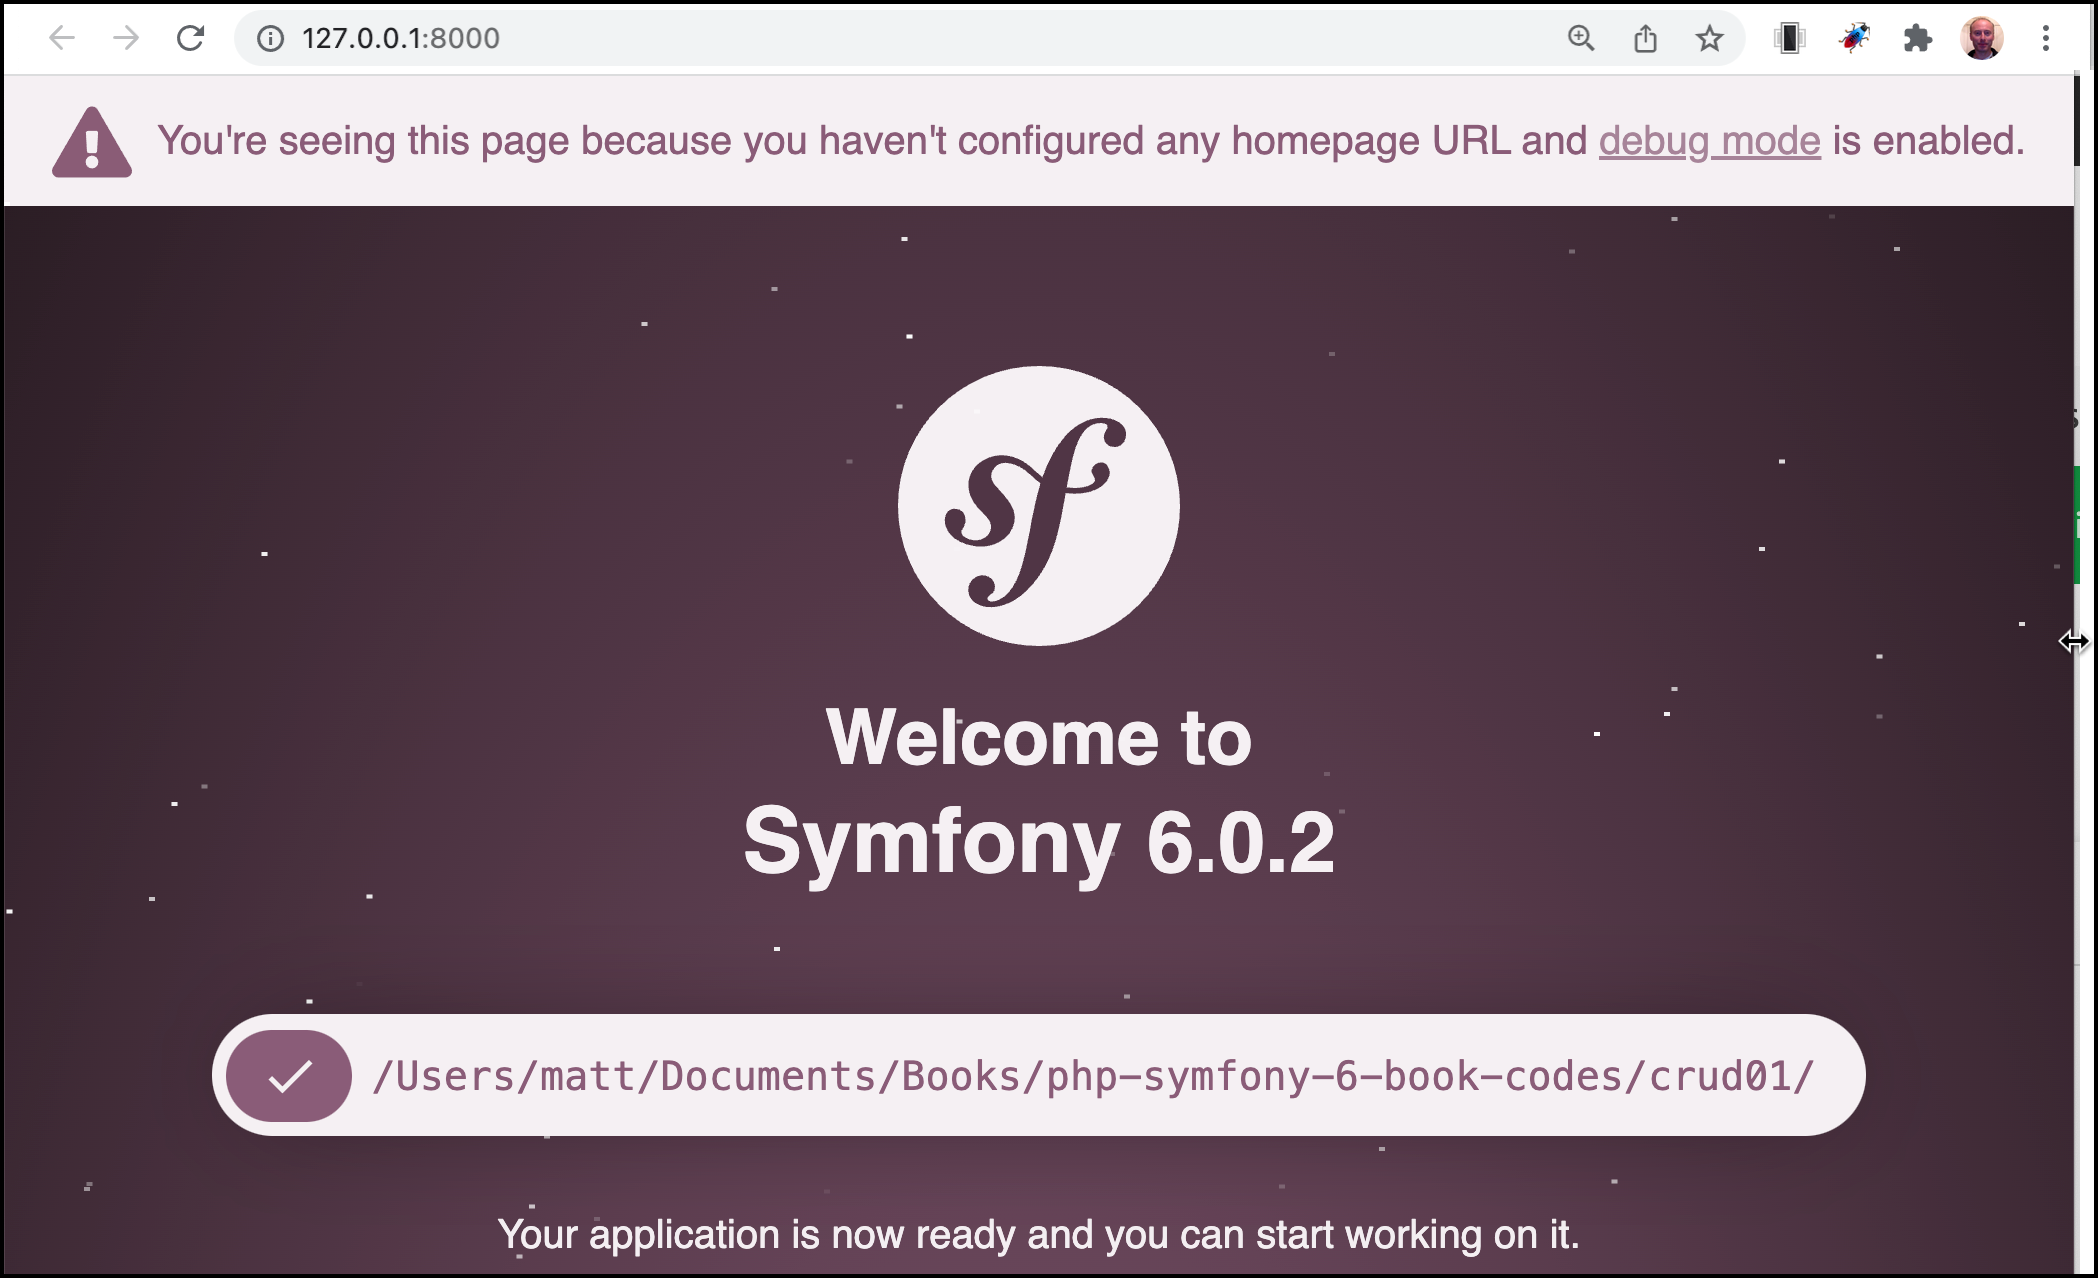
\includegraphics[width=0.75\textwidth,height=\textheight]{./tex2pdf.-2b0e1314f8bbbae5/7a430dcb3125bbcf87bbbecc80178ddec044edda.png}
\caption{Default Symfony home page. \label{homepage}}
\end{figure}

\hypertarget{connect-to-and-create-our-mysql-database}{%
\chapter{Connect to and create our MySQL
database}\label{connect-to-and-create-our-mysql-database}}

We need to set things up so our PHP web application can communicate with
MySQL and also setup our example database.

Do the following:

\begin{enumerate}
\def\labelenumi{\arabic{enumi}.}
\item
  Check the credentials in the \texttt{.env} file match your setup. If
  you are using the default MySQL server settings, the only thing you
  may need to change are the password for the \texttt{root} user:
\item
  Start up MySQL Workbench (\texttt{root} password was \texttt{Pass\$\$}
  on college computers last time I checked - you should know what ever
  root password is on your own computer - and I do recommend you HAVE a
  password for the MySQL root user \ldots{})

  \begin{itemize}
  \tightlist
  \item
    you may need to `Clear the Vault' before being able to run an
    instance of MySQL \ldots{}
  \end{itemize}
\end{enumerate}

That's it - PHP should now be able to communicate with MySQL - let's
find out \ldots{}

Tell Symfony to create its database:

\begin{Shaded}
\begin{Highlighting}[]
\NormalTok{    $ }\ExtensionTok{symfony}\NormalTok{ console doctrine:database:create}

    \ExtensionTok{Created}\NormalTok{ database }\StringTok{'crud01'}\NormalTok{ for connection named default}
\end{Highlighting}
\end{Shaded}

(or you can use the 2-letter abbreviated version:
\texttt{symfony\ console\ do:da:cr})

If you see the \texttt{created\ database} message then things are going
well.

\hypertarget{the-2019-php-mysql-issue}{%
\section{The 2019 PHP-MySQL issue}\label{the-2019-php-mysql-issue}}

NOTE:

\begin{itemize}
\item
  Due to a change in MySQL during 2019 we may need to run a special
  command in MySQL to allow PHP programs to communicate with MySQL:
\item
  in an SQL window in MySQL workbench execute the following command

\begin{Shaded}
\begin{Highlighting}[]
  \KeywordTok{alter} \FunctionTok{user} \StringTok{'root'}\NormalTok{@}\StringTok{'localhost'} \KeywordTok{identified} \KeywordTok{with}\NormalTok{ mysql_native_password }\KeywordTok{by} \StringTok{'Pass$$'}\NormalTok{;}
\end{Highlighting}
\end{Shaded}
\end{itemize}

this should solve the problem (althogh it may have been fixed in a more
recent version of MySQL/PHP \ldots{})

\hypertarget{pre--ensure-the-migrations-folder-is-empty}{%
\section{\texorpdfstring{Pre- ensure the \texttt{/migrations} folder is
empty}{Pre- ensure the /migrations folder is empty}}\label{pre--ensure-the-migrations-folder-is-empty}}

If there is a folder \texttt{/migrations} DELETE its contents (since we
have a new database, we don't want any old migrations to mess it up)

\begin{itemize}
\tightlist
\item
  but do not delete the directory itself, otherwise it will through an
  error when trying to setup the datatabase
\end{itemize}

\hypertarget{migrating-code-entities-to-db-tables}{%
\section{Migrating code Entities to DB
tables}\label{migrating-code-entities-to-db-tables}}

Now do the following:

\begin{enumerate}
\def\labelenumi{\arabic{enumi}.}
\item
  Create a new migration:

  \texttt{symfony\ console\ make:migration}

  \begin{itemize}
  \item
    (or you can use the 2-letter abbreviated version:
    \texttt{symfony\ console\ ma:mi})
  \item
    if you are curious, you are creating SQL to create DB tables for the
    classes in \texttt{/src/Entity} in this step\ldots{}, and you can
    see this created SQL code in the PHP classes created in the
    \texttt{/migrations} folder \ldots{}
  \end{itemize}
\item
  Run the migration:

  \texttt{symfony\ console\ doctrine:migrations:migrate}

  \begin{itemize}
  \item
    (or you can use the 2-letter abbreviated version:
    \texttt{symfony\ console\ do:mi:mi})

    \begin{itemize}
    \tightlist
    \item
      say \texttt{y} when asked
    \end{itemize}
  \end{itemize}
\end{enumerate}

\hypertarget{loading-initial-data-into-the-database}{%
\section{Loading initial data into the
Database}\label{loading-initial-data-into-the-database}}

Now do the following:

\begin{enumerate}
\def\labelenumi{\arabic{enumi}.}
\setcounter{enumi}{3}
\item
  Load test data (fixtures)

  \texttt{symfony\ console\ doctrine:fixtures:load}

  \begin{itemize}
  \item
    (or you can use the 2-letter abbreviated version:
    \texttt{symfony\ console\ do:fi:lo})

    \begin{itemize}
    \tightlist
    \item
      say \texttt{y} when asked
    \end{itemize}
  \item
    if you are curious, you are running the classes in
    \texttt{/src/DataFixtures} in this step\ldots{}
  \end{itemize}
\item
  Now in MySQL workbench let's see what we've created, execute SQL:

\begin{Shaded}
\begin{Highlighting}[]
   \KeywordTok{use}\NormalTok{ crud01;}

   \KeywordTok{select} \OperatorTok{*} \KeywordTok{from} \FunctionTok{user}\NormalTok{;}
\end{Highlighting}
\end{Shaded}
\end{enumerate}

See Figure \ref{db_users} shows a screenshot of our database contents in
the MySQL Workbench DB client.

\begin{figure}
\centering
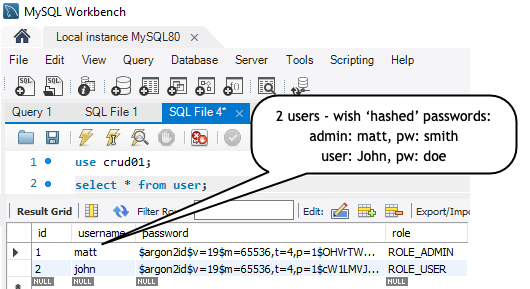
\includegraphics[width=1\textwidth,height=\textheight]{./tex2pdf.-2b0e1314f8bbbae5/990c4162a5e84b44da4e3d7eeed5f985f5c32d3f.png}
\caption{User details in the database. \label{db_users}}
\end{figure}

\hypertarget{solving-common-problems-errors-when-executing-migrations-table-already-exists-etc.}{%
\section{SOLVING COMMON PROBLEMS: Error(s) when executing MIGRATIONS
(table already exists
etc.)}\label{solving-common-problems-errors-when-executing-migrations-table-already-exists-etc.}}

Each Migration is the incremental bit of SQL that needs to be executed
to update the MySQL database structure to match our PHP Entity Classes.

Sometimes things will get out of synch - so that when we try to execute
a migration with: doctrine:migrations:migrate, we get some errors about
tables/properties already existing

The quickest and easiest way to get past this problem is to start again
with a BRAND NEW EMPTY database, and NO MIGRATIONS - do this with the
following 3 steps:

\begin{enumerate}
\def\labelenumi{\arabic{enumi}.}
\item
  Change the database name in file \texttt{.env}

  \begin{itemize}
  \tightlist
  \item
    personally I just add 1 to the number of this database, e.g.~change
    \texttt{crud01} to \texttt{crud02} and so on
  \end{itemize}
\item
  Delete all historic migrations, just delete ALL files inside folder
  \texttt{/Migrations}

  \begin{itemize}
  \tightlist
  \item
    NOTE: Do \textbf{not} delete the folder itself, otherwise you'll get
    errors when you try to create new migrations \ldots{}
  \end{itemize}
\item
  Run your steps to create new db / create SQL for migrations / run SQL
  for migrations / load any fixture data:

  \begin{itemize}
  \item
    create a new database (using the credentials in \texttt{.env}):

\begin{Shaded}
\begin{Highlighting}[]
\ExtensionTok{symfony}\NormalTok{ console doctrine:database:create}
\end{Highlighting}
\end{Shaded}
  \item
    write the SQL we need to create database to match the classes in
    \texttt{/src/Entity}:

\begin{Shaded}
\begin{Highlighting}[]
\ExtensionTok{symfony}\NormalTok{ console make:migration}
\end{Highlighting}
\end{Shaded}
  \item
    execute the SQL to create / alter the tables in the database:

\begin{Shaded}
\begin{Highlighting}[]
\ExtensionTok{symfony}\NormalTok{ console doctrine:migrations:migrate}
\end{Highlighting}
\end{Shaded}
  \item
    load any startup data defined in our \textbf{fixtures} classes:

\begin{Shaded}
\begin{Highlighting}[]
\ExtensionTok{symfony}\NormalTok{ console doctrine:fixtures:load}
\end{Highlighting}
\end{Shaded}
  \end{itemize}
\end{enumerate}

\hypertarget{explore-existing-phonemake-crud-pages}{%
\chapter{Explore existing phone/make CRUD
pages}\label{explore-existing-phonemake-crud-pages}}

\hypertarget{explore-the-crud-and-related-objects}{%
\section{Explore the CRUD and related
objects}\label{explore-the-crud-and-related-objects}}

Take a few minutes to explore the existing entities and CRUD HTML forms

\begin{itemize}
\tightlist
\item
  view the different Phone Makes
\item
  view the different Phones
\item
  see how the Make of a Phone is a link to that Make object
\item
  see how adding a new Make object means that when a Phone object is
  created/edited, that new Make appears in the dropdown list of Makes
\end{itemize}

\newpage

\hypertarget{add-make-to-end-of-url-for-phone-make-admin-pages}{%
\section{\texorpdfstring{Add \texttt{make} to end of URL for phone make
admin
pages}{Add make to end of URL for phone make admin pages}}\label{add-make-to-end-of-url-for-phone-make-admin-pages}}

Visit \texttt{localhost:8000/make} - the default for CRUD admin pages is
to add the lower case name of the entity to the end of the URL.

\begin{itemize}
\tightlist
\item
  try adding a new make or editing an existing one \ldots{}
\end{itemize}

See Figure \ref{phone_make}.

\begin{figure}
\centering
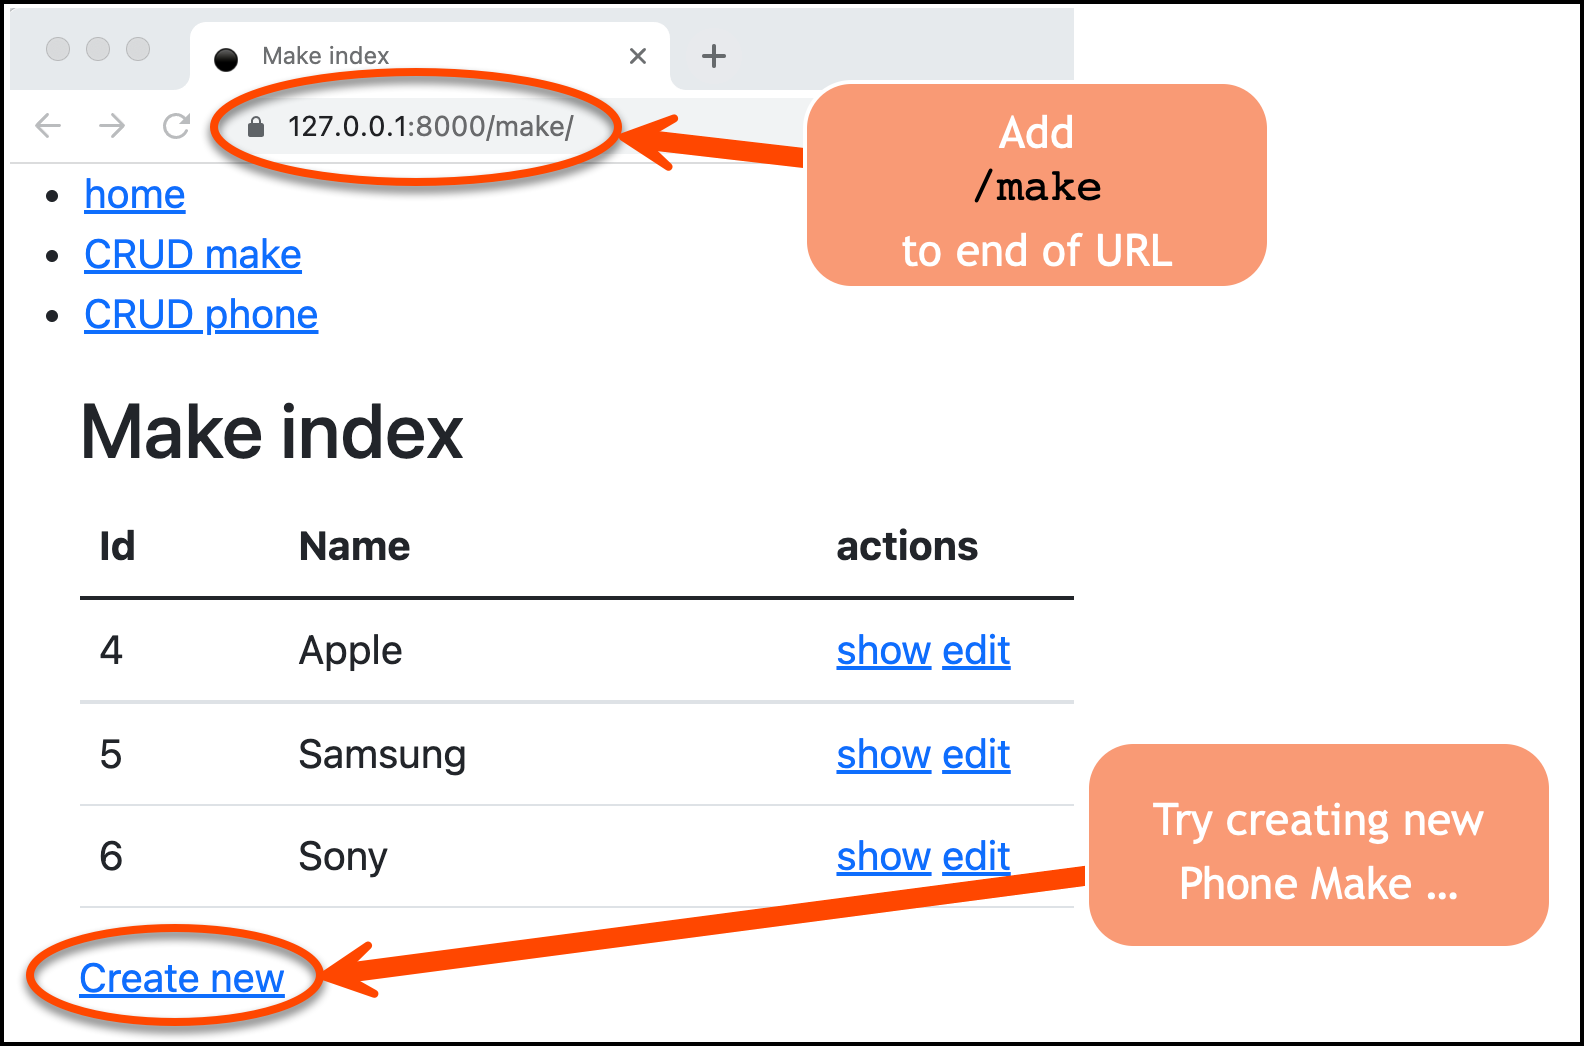
\includegraphics[width=1\textwidth,height=\textheight]{./tex2pdf.-2b0e1314f8bbbae5/589be243de6474b6ef708d87dd3912d163d0d387.png}
\caption{Screenshot of phone make CRUD pages.\label{phone_make}}
\end{figure}

\newpage

\hypertarget{browse-the-phone-records}{%
\section{Browse the Phone records}\label{browse-the-phone-records}}

Visit \texttt{localhost:8000/phone} for the Phone object admin pages -
or click the \texttt{CRUD\ phone} link:

\begin{itemize}
\tightlist
\item
  try adding a new make or editing an existing one \ldots{}
\end{itemize}

See Figure \ref{phone_index}.

\begin{figure}
\centering
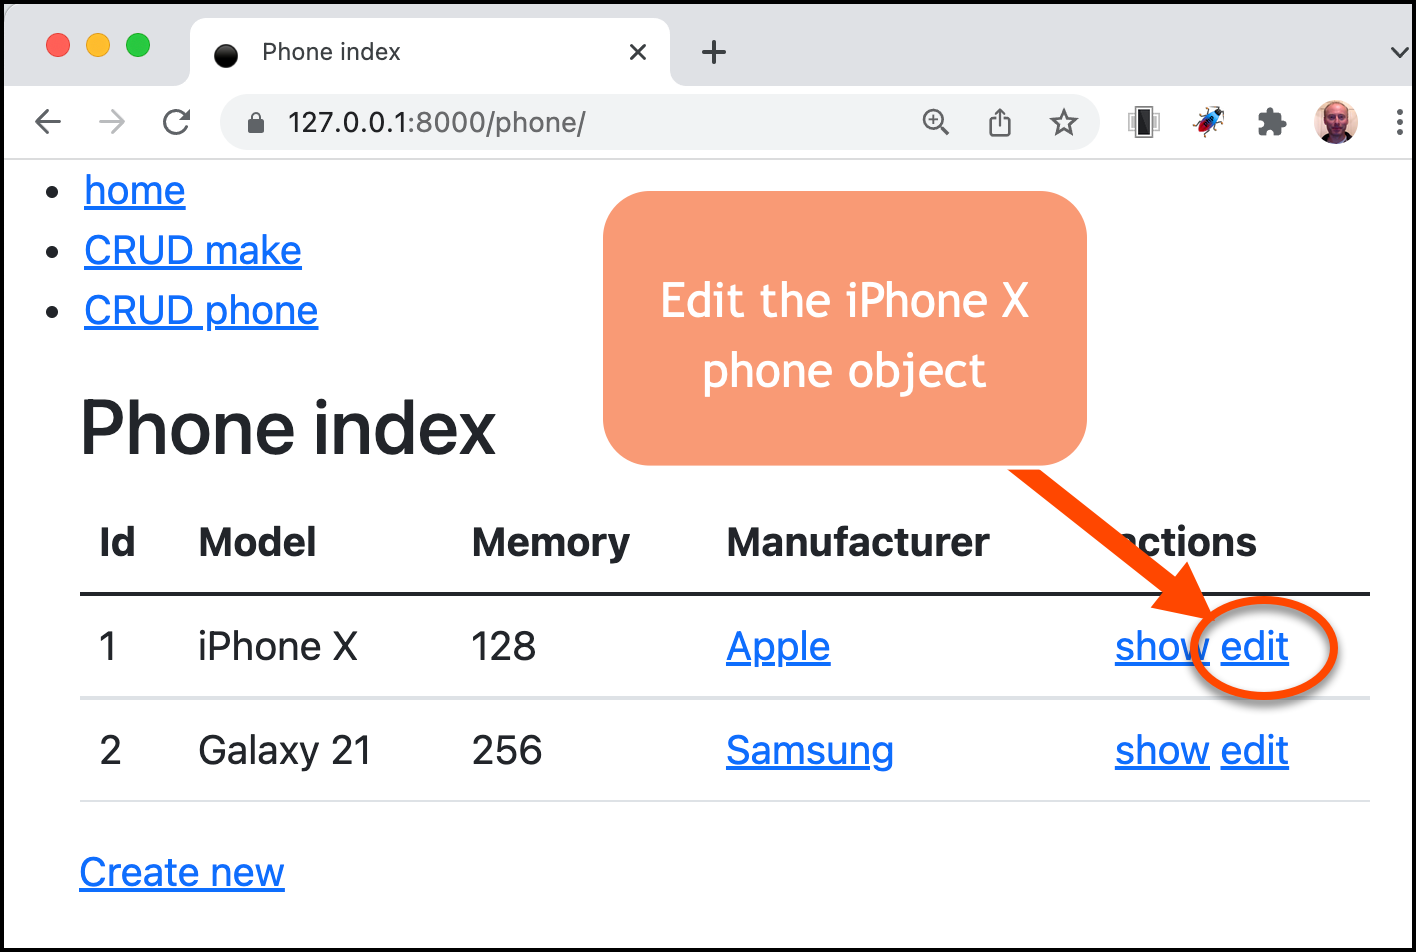
\includegraphics[width=1\textwidth,height=\textheight]{./tex2pdf.-2b0e1314f8bbbae5/2a799b2bfbfc4e78e4f9c5ad9ef60b948c664efb.png}
\caption{Screenshot of phone model CRUD pages.\label{phone_index}}
\end{figure}

\newpage

\hypertarget{many-phones-to-one-model}{%
\section{Many Phones to One Model}\label{many-phones-to-one-model}}

Edit a Phone record, and you'll see a list of the makes appear as a
drop-down list to choose from. This is a \textbf{relationship} between
each Phone object and a Phone Make object (many-to-one)

See Figure \ref{phone_edit}.

\begin{figure}
\centering
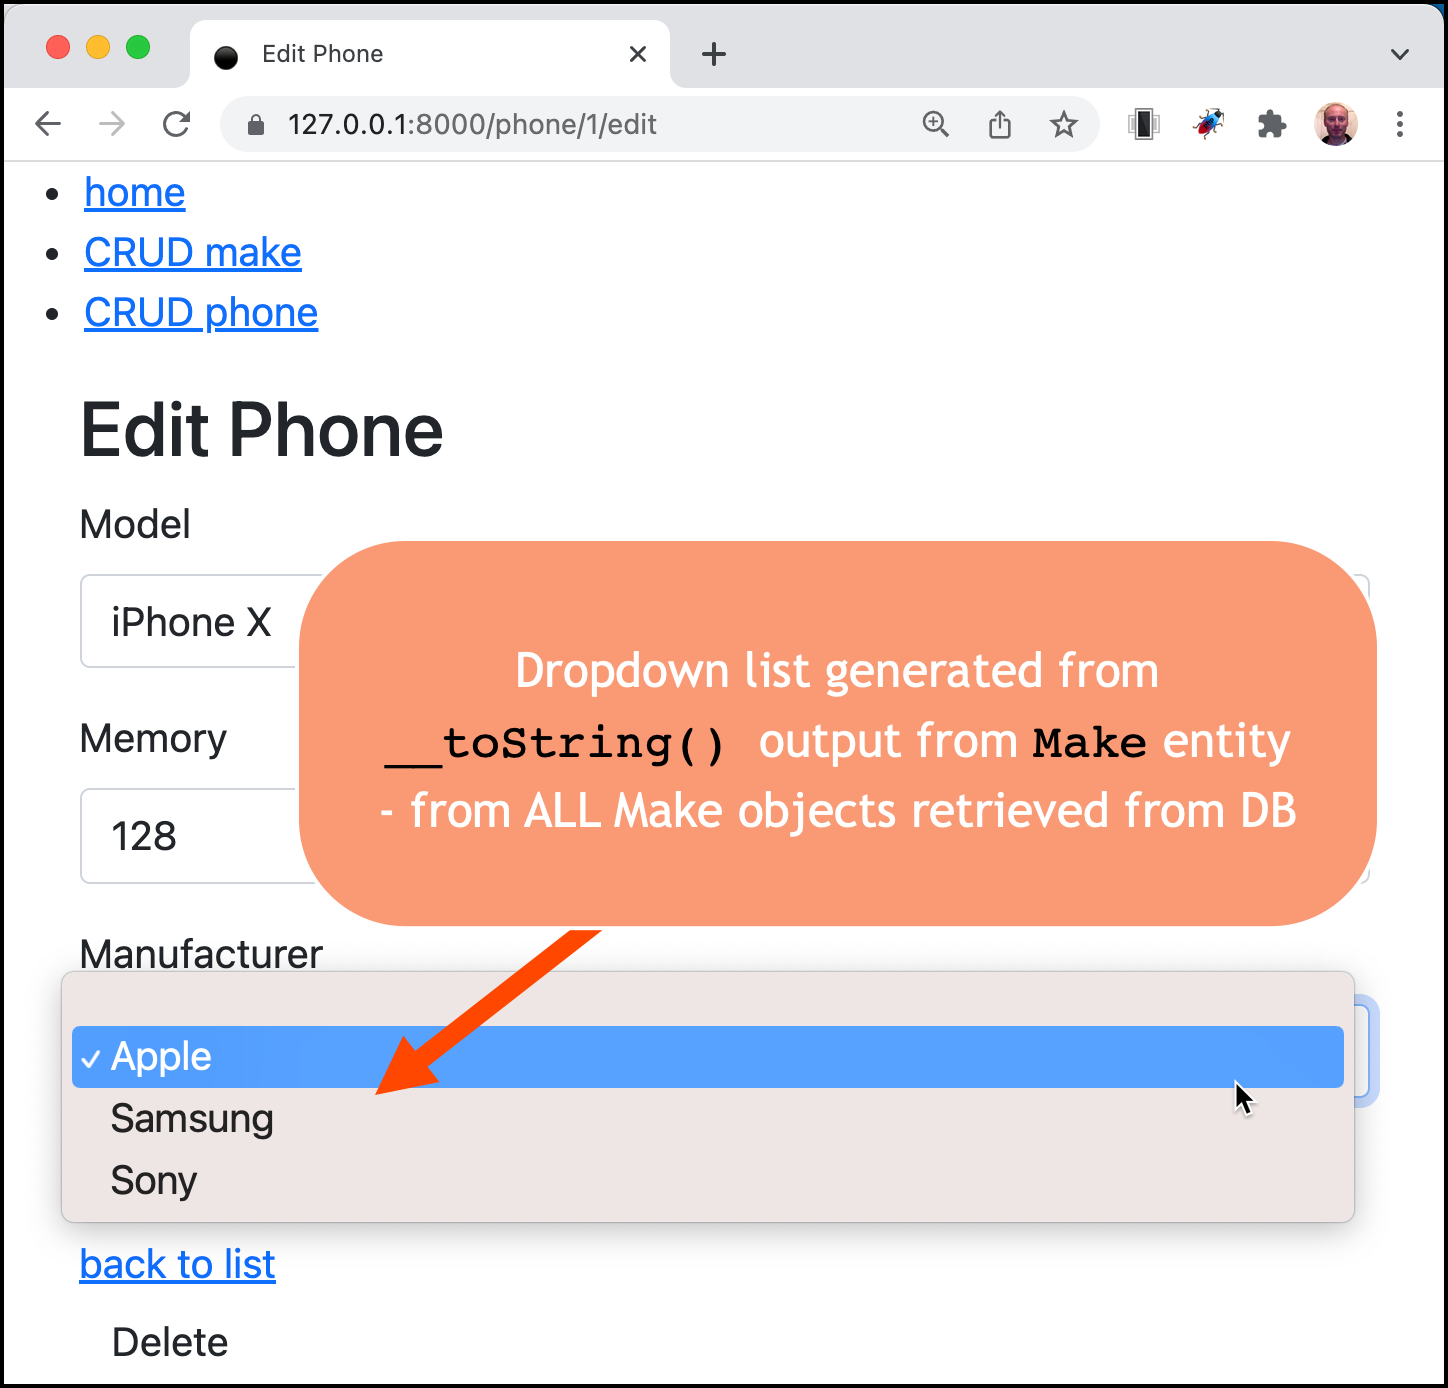
\includegraphics[width=1\textwidth,height=\textheight]{./tex2pdf.-2b0e1314f8bbbae5/f35d637c8c0cd9aaebc6b1e793c0ee9634295185.png}
\caption{Editing phone - makes as dropdown menu.\label{phone_edit}}
\end{figure}

\hypertarget{create-your-own-crud-for-a-student-entity-class}{%
\chapter{Create your own CRUD for a Student entity
class}\label{create-your-own-crud-for-a-student-entity-class}}

\hypertarget{create-student-class}{%
\section{Create Student class}\label{create-student-class}}

Let's create a Student class and generate automatic CRUD web pages.

\begin{figure}
\centering
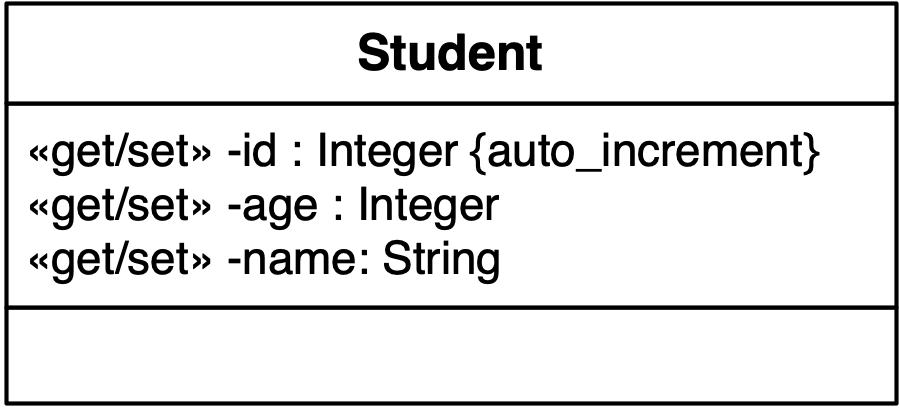
\includegraphics[width=0.75\textwidth,height=\textheight]{./tex2pdf.-2b0e1314f8bbbae5/b06182fc0ed292ee74b2047d002be6e027d35847.png}
\caption{Class diagram for Student entity.\label{student_class_diagram}}
\end{figure}

NOTE:

\begin{itemize}
\tightlist
\item
  we do \textbf{NOT} need to manually add the \texttt{id} property -
  part of the Syfony-Doctrine ORM setup is that \textbf{every} entity
  will have a single, integer, auto-increment primary-key property named
  \texttt{id}. This is \textbf{automatically} added to each new entity
  created using the \texttt{console\ make:} CLI tool.
\end{itemize}

Do the following:

\begin{enumerate}
\def\labelenumi{\arabic{enumi}.}
\item
  At the command line type:

\begin{Shaded}
\begin{Highlighting}[]
    \ExtensionTok{symfony}\NormalTok{ console make:entity Student}
\end{Highlighting}
\end{Shaded}

  You should see the following:

\begin{Shaded}
\begin{Highlighting}[]
  \OperatorTok{>} \ExtensionTok{symfony}\NormalTok{ console make:entity Student}

  \ExtensionTok{created}\NormalTok{: src/Entity/Student.php}
  \ExtensionTok{created}\NormalTok{: src/Repository/StudentRepository.php}

  \ExtensionTok{Entity}\NormalTok{ generated! Now let}\StringTok{'s add some fields!}
\StringTok{  You can always add more fields later manually or by re-running this command.}
\end{Highlighting}
\end{Shaded}

  \begin{itemize}
  \item
    notice that it tells us that is has created 2 new classes
    \texttt{src/Entity/Student.php} and
    \texttt{src/Repository/StudentRepository.php}

    \begin{itemize}
    \tightlist
    \item
      \texttt{Student.php} is a simple class with private propetries and
      getters/setters, with special `annotation' comments so these
      objects can map directly to rows in a database table\ldots{}
    \end{itemize}
  \end{itemize}
\item
  Now we need to ask this console `make' tool to add an integer
  \texttt{age} property for us:

  \begin{itemize}
  \item
    we need to enter the property name \texttt{age}
  \item
    we need to specify its data type \texttt{integer}
  \item
    (to keep things simple) we don't mind if our properties start as
    null

    \begin{itemize}
    \tightlist
    \item
      just press \texttt{\textless{}RETURN\textgreater{}} for this
      question - this accepts the offered default in these interactive
      CLI scripts \ldots{}
    \end{itemize}
  \item
    you should see the following when answering these questions at the
    \texttt{make} command tool prompt:
  \end{itemize}

\begin{Shaded}
\begin{Highlighting}[]
     \ExtensionTok{New}\NormalTok{ property name (press }\OperatorTok{<}\NormalTok{return}\OperatorTok{>}\NormalTok{ to stop adding fields)}\BuiltInTok{:}
     \OperatorTok{>} \ExtensionTok{age}

     \ExtensionTok{Field}\NormalTok{ type (enter ? to see all types) [}\ExtensionTok{string}\NormalTok{]:}
     \OperatorTok{>} \ExtensionTok{integer}

     \ExtensionTok{Can}\NormalTok{ this field be null in the database (nullable) }\KeywordTok{(}\ExtensionTok{yes/no}\KeywordTok{)}\NormalTok{ [}\ExtensionTok{no}\NormalTok{]:}
     \OperatorTok{>} 

     \ExtensionTok{updated}\NormalTok{: src/Entity/Student.php}
\end{Highlighting}
\end{Shaded}
\item
  Now add a string \texttt{name} property:

  \begin{itemize}
  \item
    we need to enter the property name \texttt{name}
  \item
    we need to specify its data type \texttt{string} (since default just
    press \texttt{\textless{}RETURN\textgreater{}})
  \item
    accept default string length of 255 (since default just press
    \texttt{\textless{}RETURN\textgreater{}})
  \item
    can be nullable (since default just press
    \texttt{\textless{}RETURN\textgreater{}})
  \item
    you should see the following when answering these questions at the
    \texttt{make} command tool prompt:
  \end{itemize}

\begin{Shaded}
\begin{Highlighting}[]
     \ExtensionTok{Add}\NormalTok{ another property? Enter the property name (or press }\OperatorTok{<}\NormalTok{return}\OperatorTok{>}\NormalTok{ to stop adding fields)}\BuiltInTok{:}
     \OperatorTok{>} \ExtensionTok{name}

     \ExtensionTok{Field}\NormalTok{ type (enter ? to see all types) [}\ExtensionTok{string}\NormalTok{]:}
     \OperatorTok{>} 

     \ExtensionTok{Field}\NormalTok{ length [255]:}
     \OperatorTok{>} 

     \ExtensionTok{Can}\NormalTok{ this field be null in the database (nullable) }\KeywordTok{(}\ExtensionTok{yes/no}\KeywordTok{)}\NormalTok{ [}\ExtensionTok{no}\NormalTok{]:}
     \OperatorTok{>} 

     \ExtensionTok{updated}\NormalTok{: src/Entity/Student.php}
\end{Highlighting}
\end{Shaded}
\item
  That's all our fields created, so just press
  \texttt{\textless{}RETURN\textgreater{}} to complete creation of our
  entity:

\begin{Shaded}
\begin{Highlighting}[]
       \ExtensionTok{Add}\NormalTok{ another property? Enter the property name (or press }\OperatorTok{<}\NormalTok{return}\OperatorTok{>}\NormalTok{ to stop adding fields)}\BuiltInTok{:}
       \OperatorTok{>} 

        \ExtensionTok{Success}\NormalTok{! }

       \ExtensionTok{Next}\NormalTok{: When you}\StringTok{'re ready, create a migration with make:migration}
\end{Highlighting}
\end{Shaded}
\end{enumerate}

\hypertarget{take-a-look-at-the-created-entity-class}{%
\section{Take a look at the created entity
class}\label{take-a-look-at-the-created-entity-class}}

Take a look at what's been created for us:
\texttt{src/Entity/Student.php}. If you ignore the comments, mostly this
is a class

See Figure \ref{student} shows a screenshot of PHPStorm and our new
class PHP code.

\begin{figure}
\centering
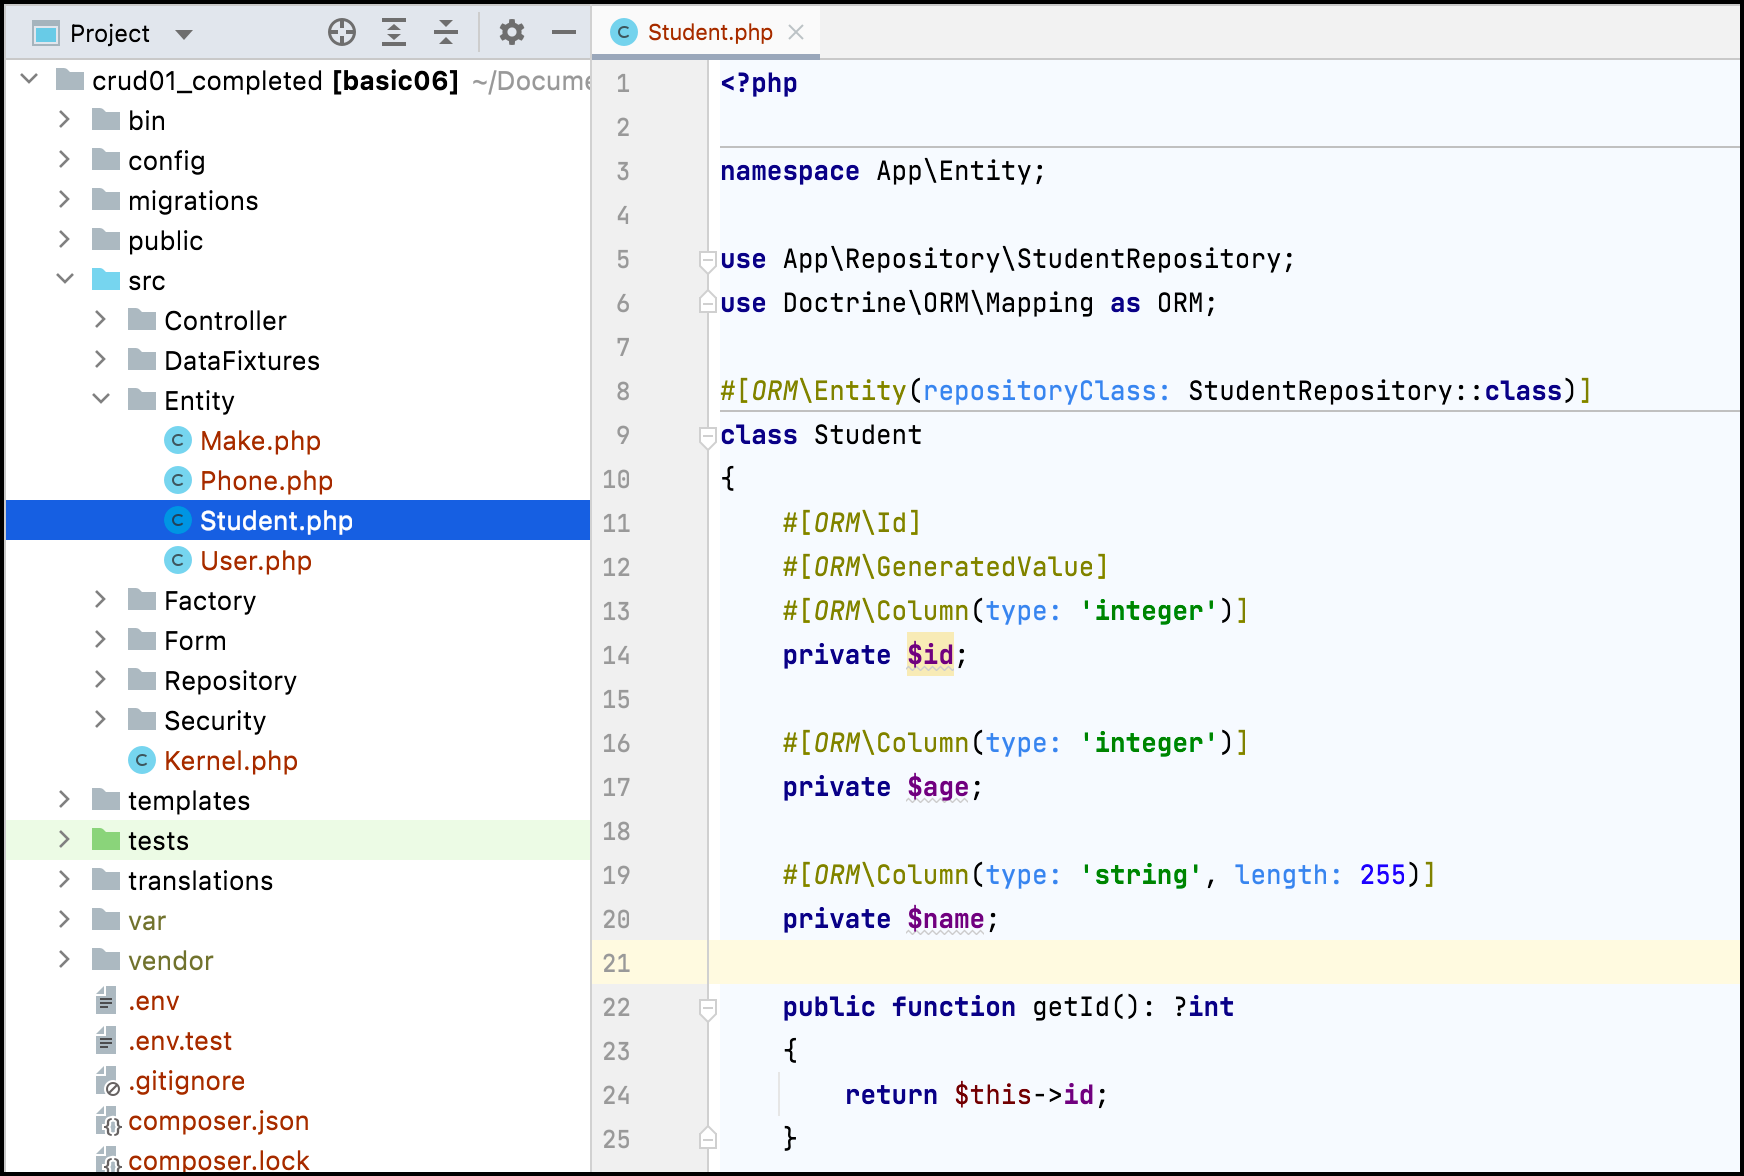
\includegraphics[width=0.9\textwidth,height=\textheight]{./tex2pdf.-2b0e1314f8bbbae5/aaf51436dc412e0d900f6fdaa3f2a64f78164437.png}
\caption{New Student.php entity. \label{student}}
\end{figure}

\hypertarget{make-migration-sql-to-create-database-to-correspond-to-our-entity-class}{%
\section{Make `migration' SQL to create database to correspond to our
entity
class}\label{make-migration-sql-to-create-database-to-correspond-to-our-entity-class}}

We can also use the `make' command line tool to look at our classes and
create the SQL commands we need to update our database create/update
tables for storing the object data in tables and rows.

Enter the following at the command line
\texttt{symfony\ console\ make:migration}

\begin{itemize}
\tightlist
\item
  or the abbreviated version: \texttt{symfony\ console\ ma:mi}
\end{itemize}

\begin{Shaded}
\begin{Highlighting}[]
    \OperatorTok{>} \ExtensionTok{symfony}\NormalTok{ console make:migration}
               
      \ExtensionTok{Success}\NormalTok{! }
    
     \ExtensionTok{Next}\NormalTok{: Review the new migration }\StringTok{"src/Migrations/Version20190927055812.php"}
     \ExtensionTok{Then}\NormalTok{: Run the migration with symfony console doctrine:migrations:migrate}
     \ExtensionTok{See}\NormalTok{ https://symfony.com/doc/current/bundles/DoctrineMigrationsBundle/index.html}
\end{Highlighting}
\end{Shaded}

If you look inside the newly created file you'll see a line like this
showing the SQL generated to create a database table to match our
\texttt{Student.php} class:

\begin{Shaded}
\begin{Highlighting}[]
    \KeywordTok{$this}\NormalTok{->addSql}\OtherTok{(}
        \StringTok{'CREATE TABLE student (}
\StringTok{            id INTEGER PRIMARY KEY AUTOINCREMENT NOT NULL, }
\StringTok{            age INTEGER NOT NULL, }
\StringTok{            name VARCHAR(255) NOT NULL}
\StringTok{            ... and some DB character set stuff ...}
\StringTok{        )'}
    \OtherTok{);}
\end{Highlighting}
\end{Shaded}

\hypertarget{execute-our-migration-sql-to-createupdate-database}{%
\section{Execute our `migration' SQL to create/update
database}\label{execute-our-migration-sql-to-createupdate-database}}

Now let's tell Symfony to connect to the database and execute the
migration SQL - to actually \textbf{create} the new \texttt{Student}
table in the database.

We need to enter the terminal command
\texttt{symfony\ console\ doctrine:migrations:migrate}:

\begin{Shaded}
\begin{Highlighting}[]
    \OperatorTok{>} \ExtensionTok{symfony}\NormalTok{ console doctrine:migrations:migrate}
                                                                  
        \ExtensionTok{Application}\NormalTok{ Migrations                    }
                                                                  
    \ExtensionTok{WARNING}\NormalTok{! You are about to execute a database migration that could result in schema changes and data loss. }
    \ExtensionTok{Are}\NormalTok{ you sure you wish to continue? (y/n)}
\end{Highlighting}
\end{Shaded}

At this point we must enter \texttt{y} to go ahead - saying we are happy
for our database structure to be chagned by exectuing our migration SQL:

\begin{Shaded}
\begin{Highlighting}[]
    \ExtensionTok{WARNING}\NormalTok{! You are about to execute a database migration that could result in schema changes and data loss. }
    \ExtensionTok{Are}\NormalTok{ you sure you wish to continue? (y/n)}\ExtensionTok{y}

    \ExtensionTok{Migrating}\NormalTok{ up to 20190927055812 from 0}
    
      \ExtensionTok{++}\NormalTok{ migrating 20190927055812}
         \ExtensionTok{-}\OperatorTok{>}\NormalTok{ CREATE TABLE student (id INTEGER PRIMARY KEY AUTOINCREMENT NOT NULL, }
        \ExtensionTok{age}\NormalTok{ INTEGER NOT NULL, name VARCHAR(255) }\ExtensionTok{NOT}\NormalTok{ NULL)}
    
      \ExtensionTok{++}\NormalTok{ migrated (took 64.4ms, used 18M memory)}
      \ExtensionTok{------------------------}
      \ExtensionTok{++}\NormalTok{ finished in 70.8ms}
      \ExtensionTok{++}\NormalTok{ used 18M memory}
      \ExtensionTok{++}\NormalTok{ 1 migrations executed}
      \ExtensionTok{++}\NormalTok{ 1 sql queries}
\end{Highlighting}
\end{Shaded}

That's it - we have now created a table in out database to match our PHP
entity class.

\hypertarget{generate-the-crud-web-form-for-class-student}{%
\section{\texorpdfstring{Generate the \textbf{CRUD} web form for class
\texttt{Student}}{Generate the CRUD web form for class Student}}\label{generate-the-crud-web-form-for-class-student}}

Let's generate some HTML and PHP code for a web form to list and
create-read-update-delete data from our database.

We need to execute this command to create that code
\texttt{symfony\ console\ make:crud\ Student}:

\begin{itemize}
\tightlist
\item
  press \texttt{\textless{}RETURN\textgreater{}} to accept the default
  controller class name of \texttt{StudentController}:
\end{itemize}

\begin{Shaded}
\begin{Highlighting}[]
    \OperatorTok{>} \ExtensionTok{symfony}\NormalTok{ console make:crud Student}
    
      \ExtensionTok{Choose}\NormalTok{ a name for your controller class (e.g. StudentController) [}\ExtensionTok{StudentController}\NormalTok{]:}
       \OperatorTok{>}               \KeywordTok{(}\ExtensionTok{press} \OperatorTok{<}\NormalTok{RETURN}\OperatorTok{>}\NormalTok{ here to accept default offered}\KeywordTok{)}

     \ExtensionTok{created}\NormalTok{: src/Controller/StudentController.php}
     \ExtensionTok{created}\NormalTok{: src/Form/StudentType.php}
     \ExtensionTok{created}\NormalTok{: templates/student/_delete_form.html.twig}
     \ExtensionTok{created}\NormalTok{: templates/student/_form.html.twig}
     \ExtensionTok{created}\NormalTok{: templates/student/edit.html.twig}
     \ExtensionTok{created}\NormalTok{: templates/student/index.html.twig}
     \ExtensionTok{created}\NormalTok{: templates/student/new.html.twig}
     \ExtensionTok{created}\NormalTok{: templates/student/show.html.twig}
               
      \ExtensionTok{Success}\NormalTok{! }

     \ExtensionTok{Next}\NormalTok{: Check your new CRUD by going to /student/}
\end{Highlighting}
\end{Shaded}

\hypertarget{visit-our-generated-student-crud-pages-at-student}{%
\section{\texorpdfstring{Visit our generated \texttt{Student} crud pages
at
\texttt{/student}}{Visit our generated Student crud pages at /student}}\label{visit-our-generated-student-crud-pages-at-student}}

Let's visit our generated CRUD pages, these can be found by adding
\texttt{/student} at the end of the URL.

If you stopped the server previously, run the web server again with:
\texttt{symfony\ serve}.

Click \texttt{Create\ new} and add a student. Then try clicking edit,
and change some values or delete it and create it again.

You should find you have a fully working web-based CRUD interface to
your database.

See Figure \ref{student_list} shows a screenshot of several students
having been created (and yes, one of my grandmothers did live to 96!).

\begin{figure}
\centering
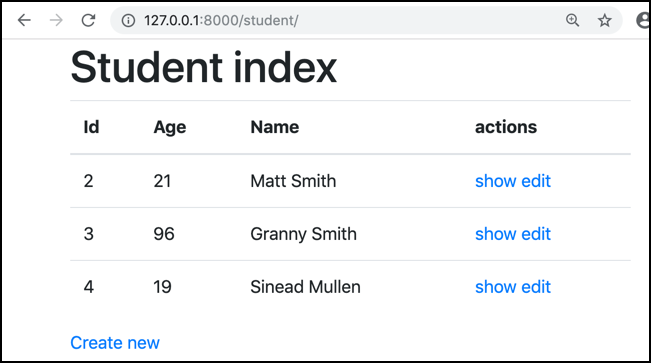
\includegraphics[width=0.75\textwidth,height=\textheight]{./tex2pdf.-2b0e1314f8bbbae5/413bb0447c351895d20b9303f385a53ed285ce1c.png}
\caption{Screenshot of nice lookling Bootstrap style admin CRUD pages.
\label{student_list}}
\end{figure}

\hypertarget{databases-are-persistent}{%
\section{\texorpdfstring{Databases are
\textbf{persistent}}{Databases are persistent}}\label{databases-are-persistent}}

Kill the Symfony web server at the command line by pressing
\texttt{\textless{}CTRL\textgreater{}-C}. Then quit the PHPStorm IDE
application.

You could also go have a cup of coffee, or perhaps shut down and restart
your computer.

Then restart the PHPStorm editor, and restart the web server with:

\begin{Shaded}
\begin{Highlighting}[]
    \ExtensionTok{symfony}\NormalTok{ serve}
\end{Highlighting}
\end{Shaded}

Now open a web browser to URL \texttt{http://localhost:8000/student} and
you should see that the students you created in your database are still
there.

Any changes we make are remembered (persisted) as part of our database.

\hypertarget{adding-a-campus-entity-and-relating-it-to-student}{%
\chapter{Adding a campus entity and relating it to
Student}\label{adding-a-campus-entity-and-relating-it-to-student}}

\hypertarget{create-a-new-class-campus}{%
\section{Create a new class: Campus}\label{create-a-new-class-campus}}

Figure \ref{campus_class_diagram} shows a class diagram for a
\texttt{Campus} entity class.

\begin{figure}
\centering
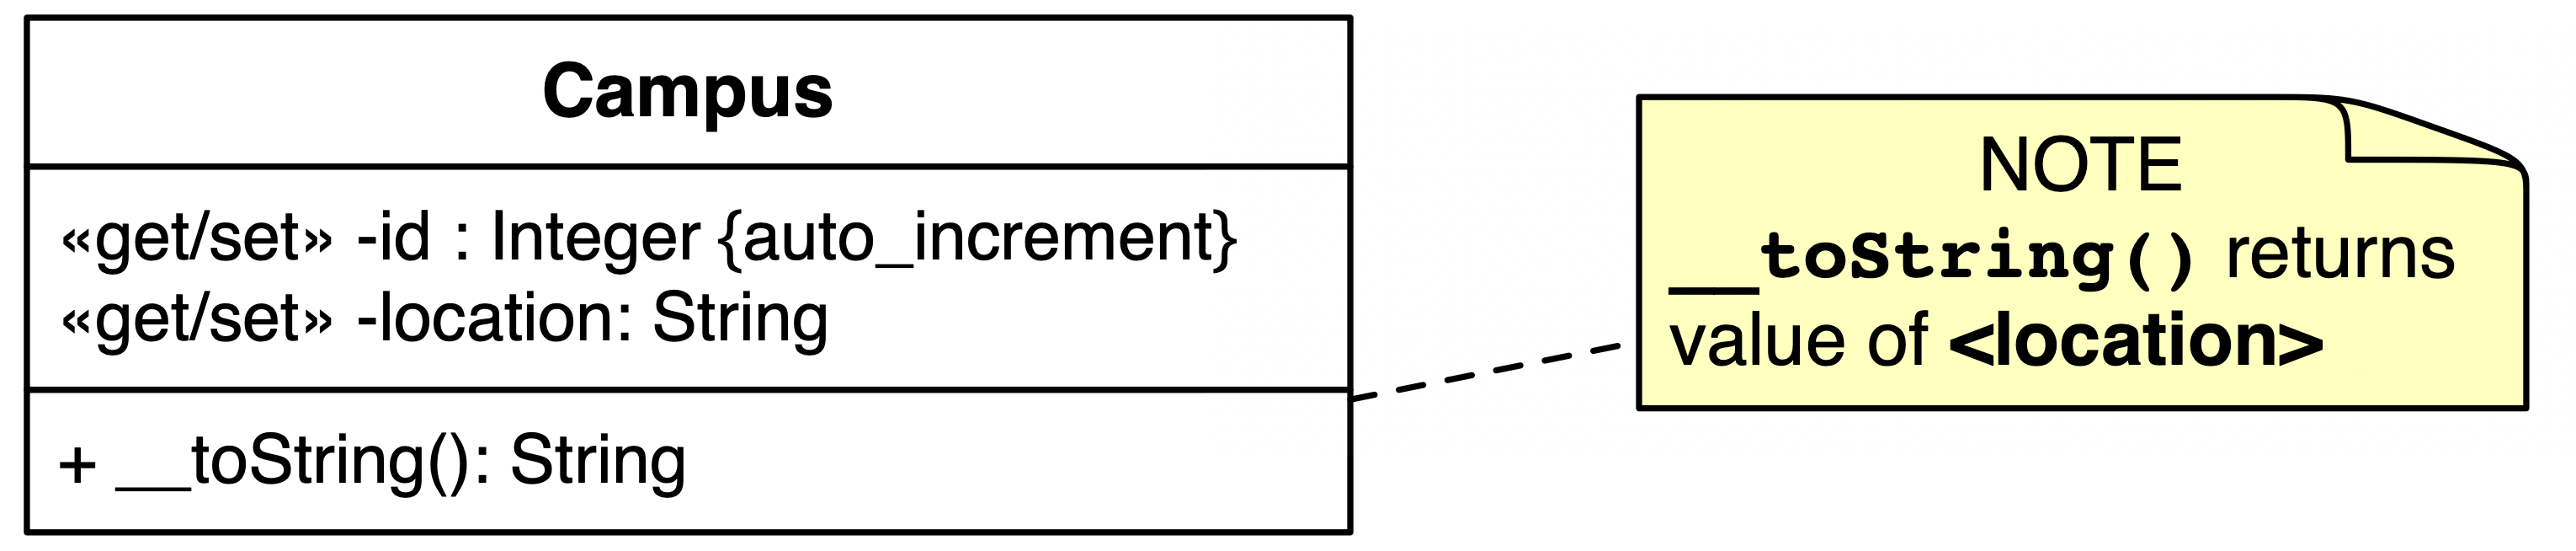
\includegraphics[width=1\textwidth,height=\textheight]{./tex2pdf.-2b0e1314f8bbbae5/80f2f3cd8caabc570fcf1ded7463dba5c252e430.png}
\caption{Class diagram for \texttt{Campus}
class.\label{campus_class_diagram}}
\end{figure}

Create entity \texttt{Campus} with single property `location' (string)
HINT:

\begin{itemize}
\item
  use the interactive command line entity maker:

  \begin{itemize}
  \tightlist
  \item
    \texttt{symfony\ console\ make:entity\ Campus}
  \item
    and add a (default type) string property named \texttt{location}
  \end{itemize}
\end{itemize}

\hypertarget{add-__tostring-method-to-campus-entity-class}{%
\section{\texorpdfstring{Add \texttt{\_\_toString()} method to
\texttt{Campus} entity
class}{Add \_\_toString() method to Campus entity class}}\label{add-__tostring-method-to-campus-entity-class}}

Now add a \texttt{\_\_toString()} method to Campus class
(\texttt{src/Entity/Campus.php}) containing the following

\begin{Shaded}
\begin{Highlighting}[]
    \KeywordTok{public} \KeywordTok{function} \FunctionTok{__toString}\OtherTok{()}\NormalTok{: }\KeywordTok{string}
\NormalTok{    \{}
        \KeywordTok{return} \KeywordTok{$this}\NormalTok{->location}\OtherTok{;}
\NormalTok{    \}}
\end{Highlighting}
\end{Shaded}

We'll need this \texttt{\_\_toString} method in \texttt{Campus} later,
so that when creating/editing \texttt{Student}s we can choose the
related \texttt{Campus} object from a \textbf{drop-down menu} - which
needs a string description of each \texttt{Campus}.

\hypertarget{generate-crud-for-this-campus-class}{%
\section{Generate CRUD for this Campus
class}\label{generate-crud-for-this-campus-class}}

Generate CRUD for Campus:

\begin{Shaded}
\begin{Highlighting}[]
\NormalTok{    $ }\ExtensionTok{symfony}\NormalTok{ console make:crud Campus}
\end{Highlighting}
\end{Shaded}

You'll see a new controller class, and some tempaltes in a folder
\texttt{templates/campus}.

\hypertarget{relate-each-student-to-one-campus}{%
\section{Relate each Student to one
Campus}\label{relate-each-student-to-one-campus}}

Figure \ref{relationship_diagram} shows the two classes related. Each
\texttt{Student} is related to exactly 1 \texttt{Campus} object, while
each \texttt{Campus} object can be related to 0 or 1 or many
\texttt{Student} objects.

\begin{figure}
\centering
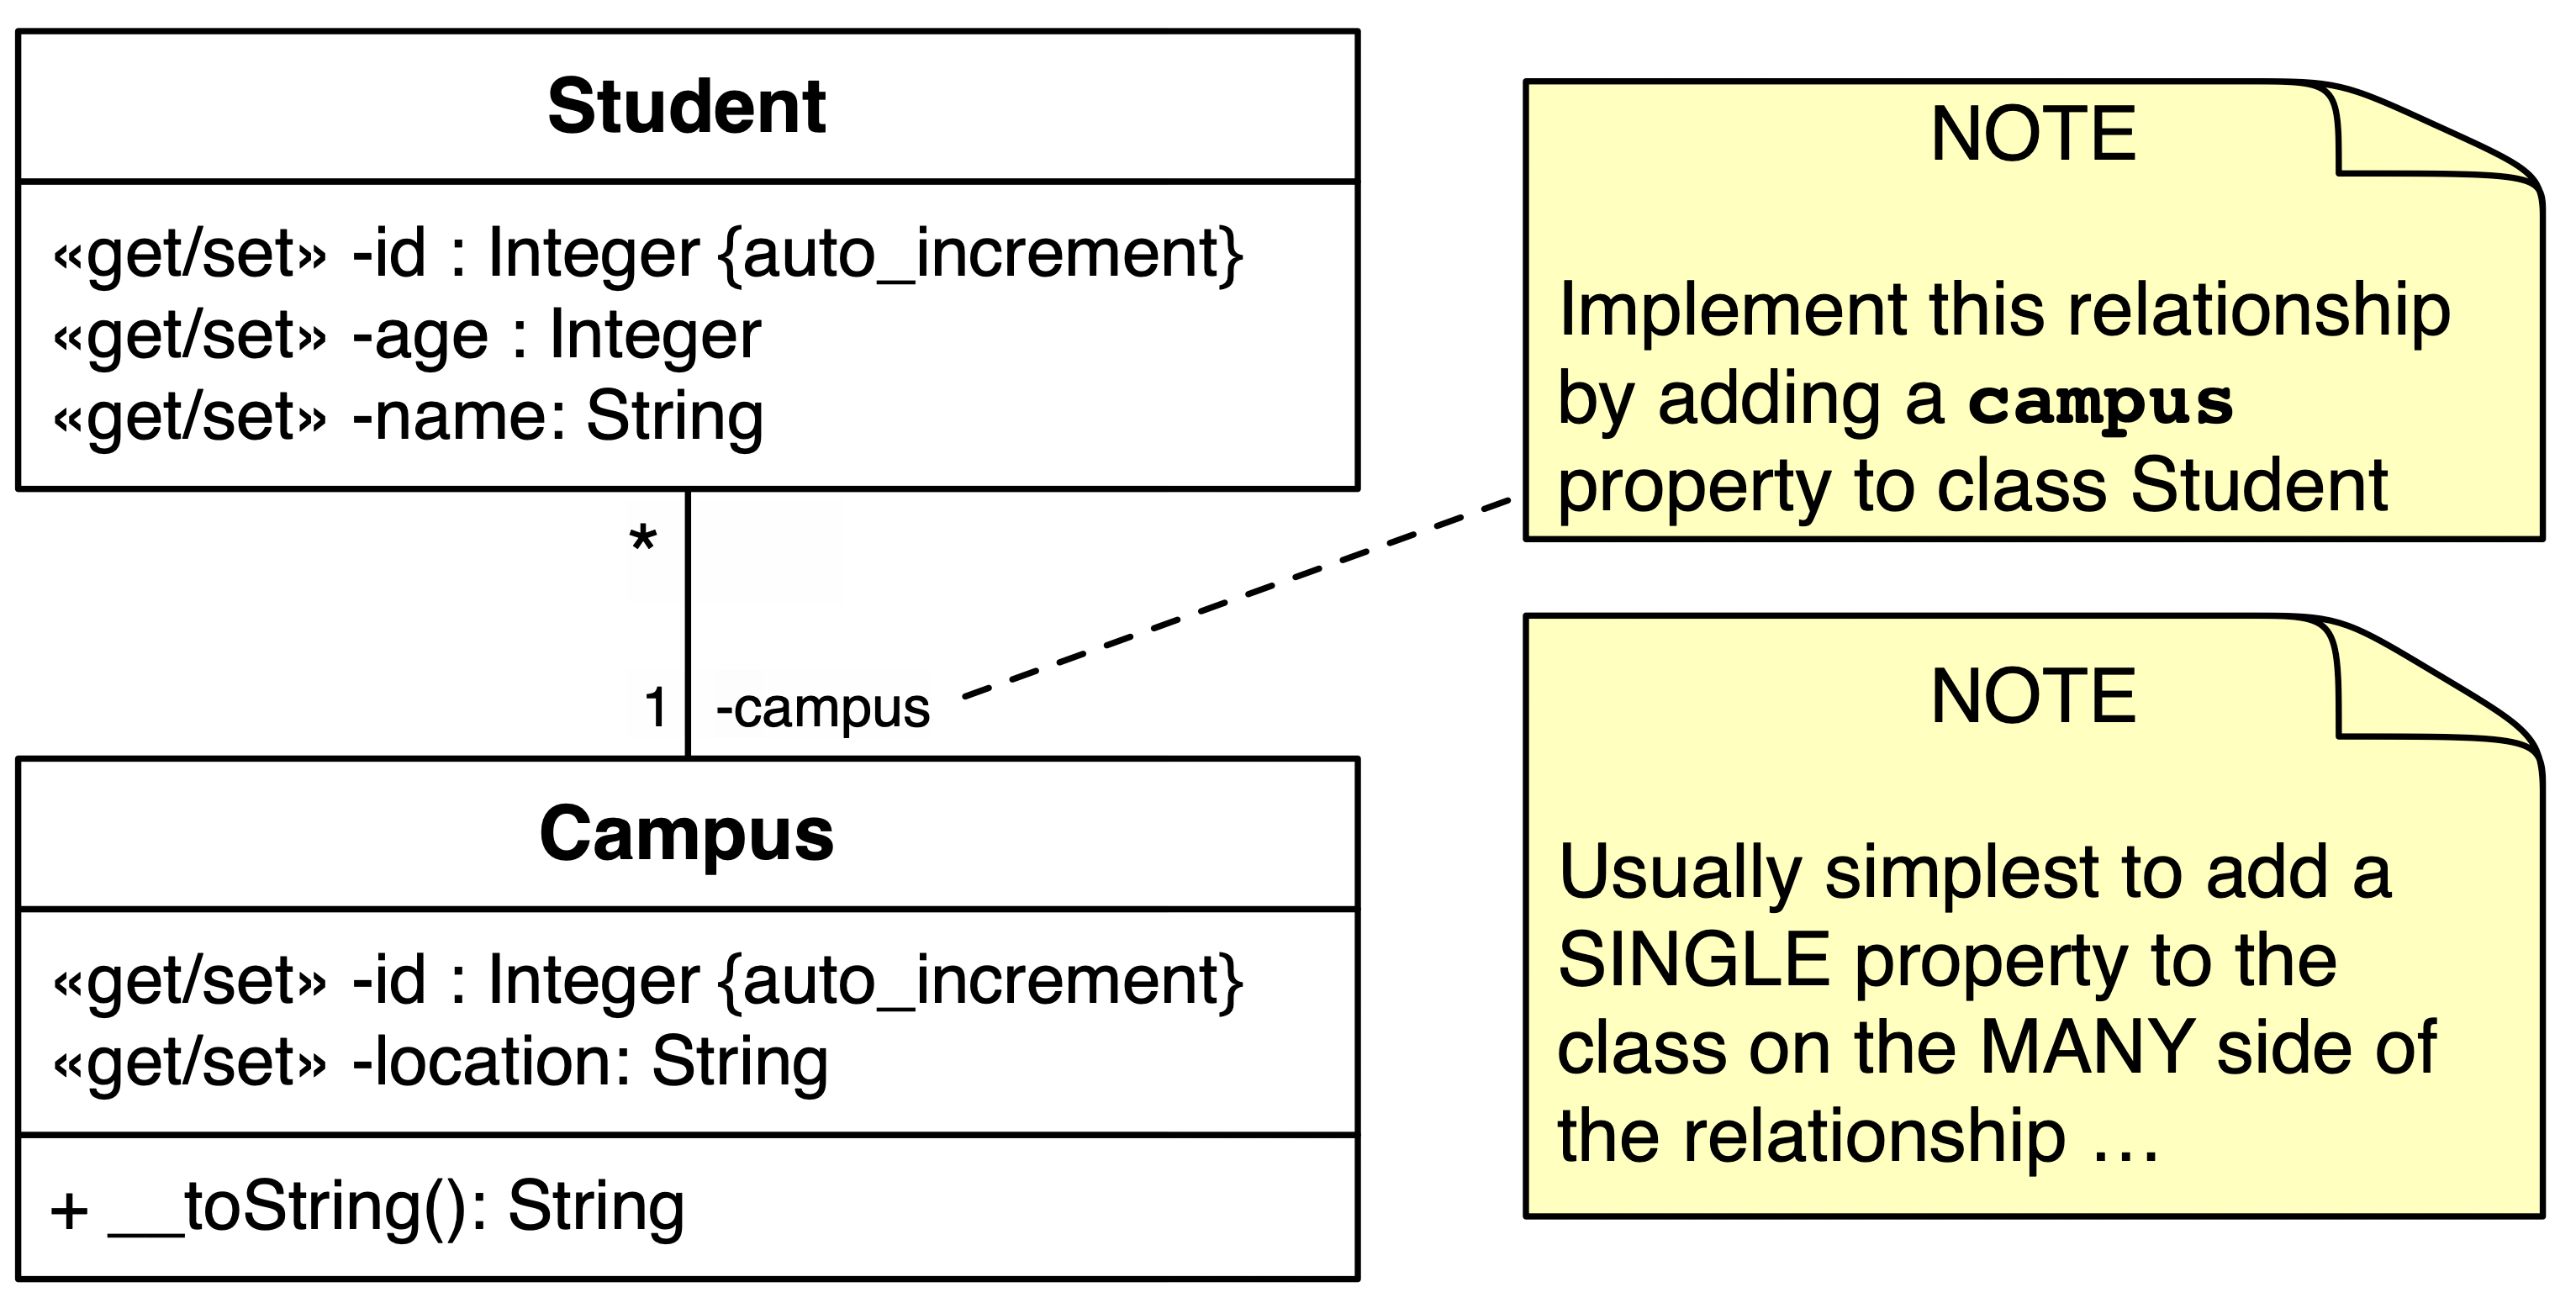
\includegraphics[width=1\textwidth,height=\textheight]{./tex2pdf.-2b0e1314f8bbbae5/aab43016ca92f606223ed7ec25a287137c41efb1.png}
\caption{Class diagram for \texttt{Student}-\texttt{Campus}
multiplicity.\label{relationship_diagram}}
\end{figure}

To create this relationship we are going to add a \textbf{`campus'}
property to the \texttt{Student} class, that is a reference to a
\texttt{Campus} object. Here is our detailed new \texttt{Student} class
diagram:

\begin{figure}
\centering
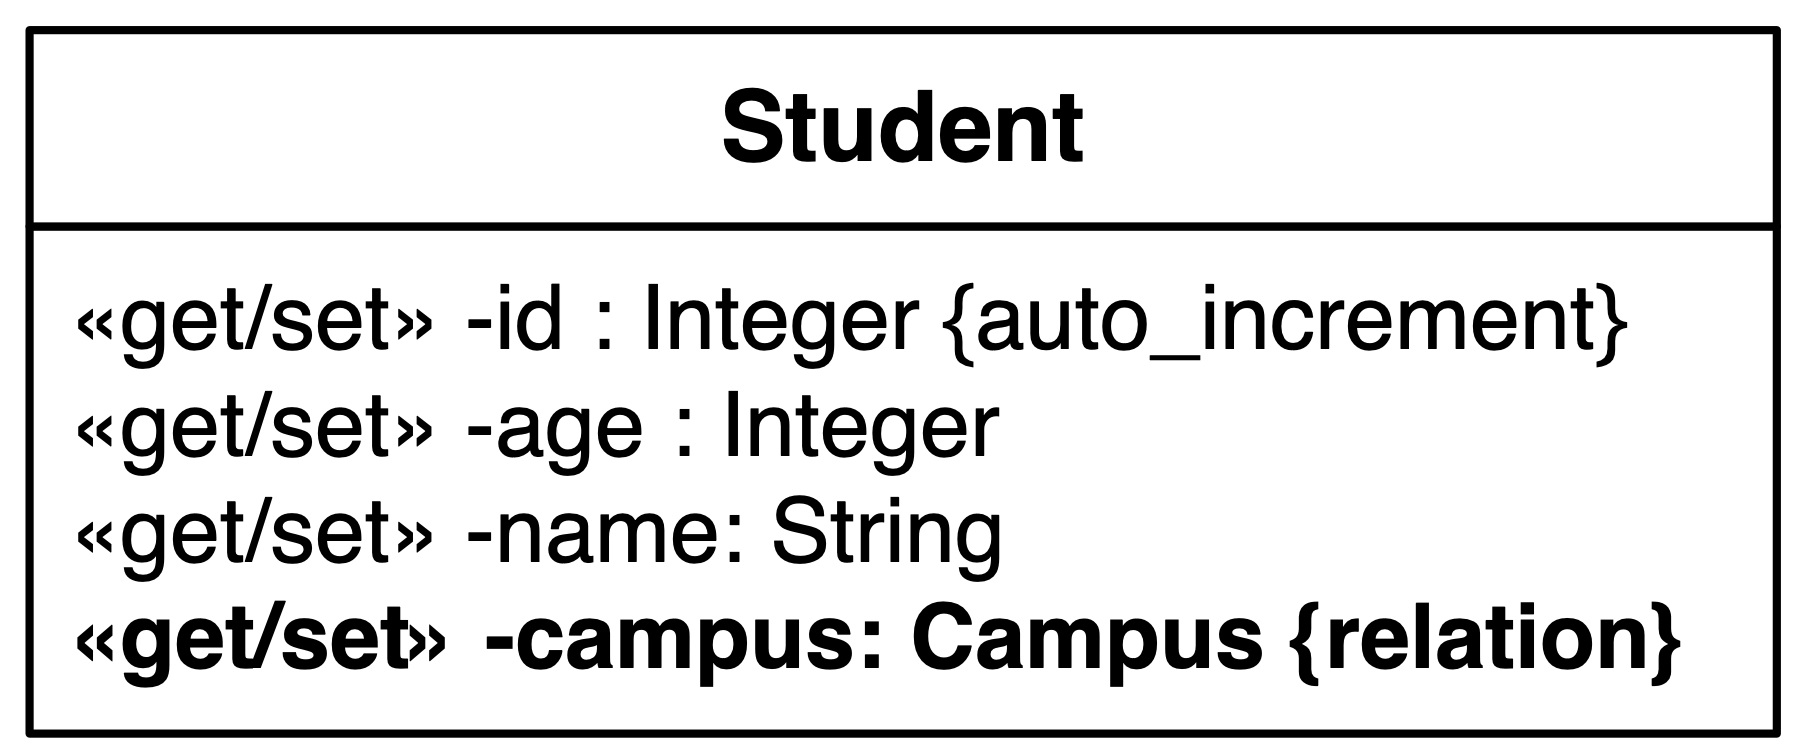
\includegraphics[width=0.75\textwidth,height=\textheight]{./tex2pdf.-2b0e1314f8bbbae5/6b159751d9c0958cc96a4f18f6854eecfebbcd1c.png}
\caption{\texttt{Student} class diagram showing implemented relationship
to \texttt{Campus} via new property
\texttt{campus}.\label{student_related_diagram}}
\end{figure}

Here is how to add a related property to a class:

\begin{itemize}
\tightlist
\item
  add a property \textbf{\texttt{campus}} to the \texttt{Student} class,
  of type \texttt{relation}

  \begin{itemize}
  \tightlist
  \item
    that is \texttt{ManyToOne} to the Campus class
  \item
    i.e.~many students linked to one campus
  \end{itemize}
\item
  to ADD a property to an existing class, we need to run the
  \texttt{make:entity} console command again:
\end{itemize}

\begin{Shaded}
\begin{Highlighting}[]
\ExtensionTok{symfony}\NormalTok{ console make:entity Student}
\end{Highlighting}
\end{Shaded}

the console should see the entity already exists, and invite us to add a
new property\ldots{}

NOTE:

\begin{itemize}
\item
  once you've given the property name, type, class, and
  \texttt{ManyToOne} relationship type, just keep hitting
  \texttt{\textless{}RETURN\textgreater{}} to accept the defaults

  \begin{itemize}
  \item
    Symfony will also add a \texttt{students} array property to the
    \texttt{Campus} class for you - that's fine

    \begin{itemize}
    \tightlist
    \item
      it's often handy, so if we have a reference to a \texttt{Campus}
      object then, for free, we get a property that is an array to all
      \texttt{Student} objects related to that \texttt{Campus}
    \end{itemize}
  \end{itemize}
\end{itemize}

NOTE: very IMPORTANT - property type is \textbf{relation} not
\textbf{string}

\begin{itemize}
\item
  do \textbf{NOT} create \textbf{string} property type for
  \texttt{campus}
\item
  the type for property \texttt{campus} must be \textbf{relation}

  \begin{itemize}
  \item
    this means the SQL generated in the migration will implement an SQL
    FOREIGN-KEY using the \textbf{id}s of Campus objects stored in a
    \texttt{campus\_id} TABLE field for table \texttt{student}
  \item
    look at the generated SQL when you make the \textbf{migration} after
    adding this relation property to campus
  \end{itemize}
\item
  if it's a string, then it won't link to a \texttt{Campus} object and
  things will not work later on \ldots{}
\end{itemize}

\hypertarget{update-database-structure-since-we-changed-our-classes}{%
\section{Update Database Structure (since we changed our
classes)}\label{update-database-structure-since-we-changed-our-classes}}

Create and run new DB migration

\begin{enumerate}
\def\labelenumi{\arabic{enumi}.}
\item
  Create a migration by typing:

\begin{Shaded}
\begin{Highlighting}[]
\ExtensionTok{symfony}\NormalTok{ console make:migration}
\end{Highlighting}
\end{Shaded}
\item
  now run the migration by typing:

\begin{Shaded}
\begin{Highlighting}[]
\ExtensionTok{symfony}\NormalTok{ console doctrine:migrations:migrate}
\end{Highlighting}
\end{Shaded}
\end{enumerate}

\hypertarget{delete-old-crud-and-generate-new-crud-for-both-classes}{%
\section{Delete old CRUD and generate new CRUD for both
classes}\label{delete-old-crud-and-generate-new-crud-for-both-classes}}

After having updated the structure of the \texttt{Student} entity class
by adding the \texttt{campus} property, we now need to re-generate the
HTML CRUD.

See Figure \ref{delete_crud} - we must remove the \textbf{old} CRUD
files, and generate new CRUD, for things to now work with the
relationship between \texttt{Student} and \texttt{Campus}.

NOTE: This is an \textbf{important step} - if you don't delete the old
CRUD files, you won't be able to generate new CRUD making use of this
relationship.

\begin{enumerate}
\def\labelenumi{\arabic{enumi}.}
\tightlist
\item
  delete the old Student CRUD

  \begin{itemize}
  \tightlist
  \item
    FILE: \texttt{src/Controller/StudentController.php}
  \item
    FILE: \texttt{src/Form/StudentType.php}
  \item
    folder: \texttt{templates/student}
  \end{itemize}
\item
  generate CRUD for Student
\end{enumerate}

\begin{Shaded}
\begin{Highlighting}[]
\ExtensionTok{symfony}\NormalTok{ console make:crud Student}
\end{Highlighting}
\end{Shaded}

\begin{figure}
\centering
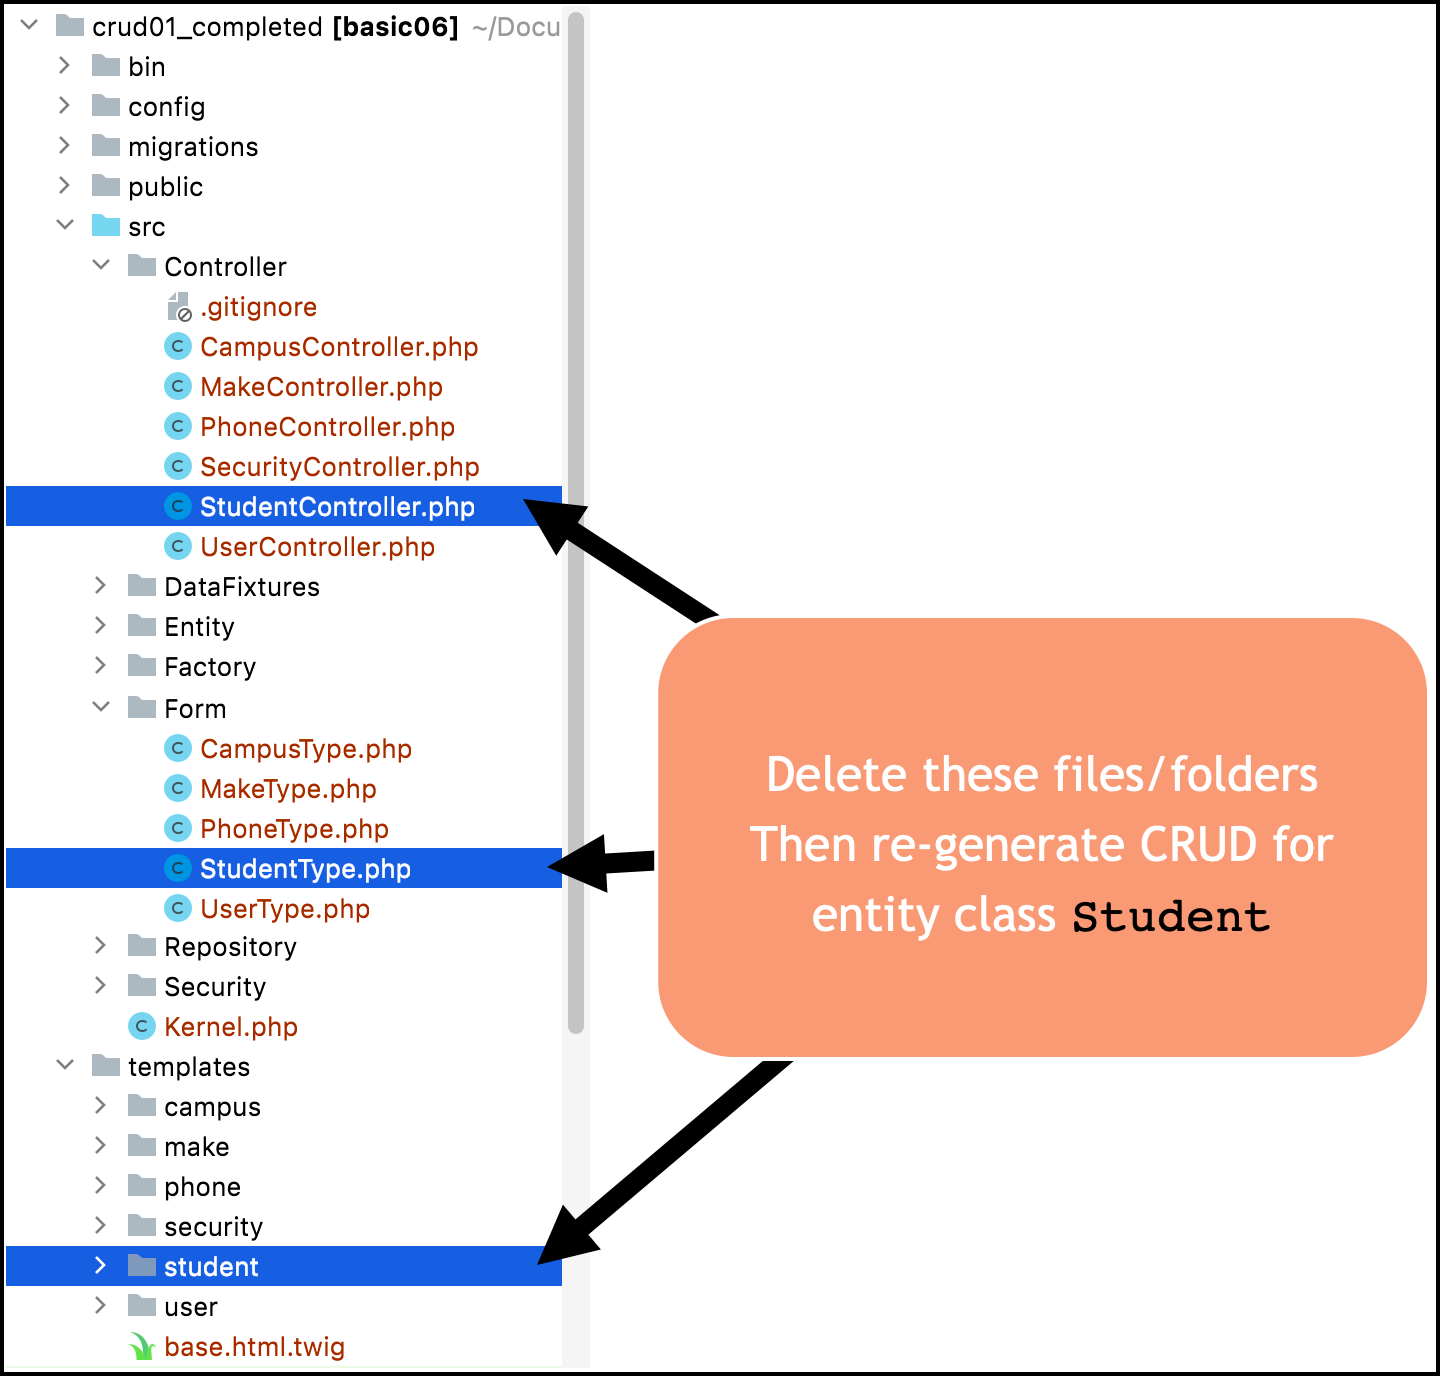
\includegraphics[width=1\textwidth,height=\textheight]{./tex2pdf.-2b0e1314f8bbbae5/784a3214b2c9d666848fc3381f2941d84684d258.png}
\caption{Deleting old Student CRUD files.\label{delete_crud}}
\end{figure}

\hypertarget{run-server-add-some-related-records}{%
\section{Run server add some related
records:}\label{run-server-add-some-related-records}}

\begin{enumerate}
\def\labelenumi{\arabic{enumi}.}
\item
  now run server:

\begin{Shaded}
\begin{Highlighting}[]
    \ExtensionTok{symfony}\NormalTok{ serve}
\end{Highlighting}
\end{Shaded}
\item
  visit the \texttt{Campus} CRUD pages and create record for 2 campuses

  \begin{itemize}
  \tightlist
  \item
    e.g.~\textbf{Blanch} and \textbf{Tallaght}
  \end{itemize}
\item
  visit the \texttt{Student} CRUD pages, and edit / create Student's
  related to your new Campuses
\end{enumerate}

\begin{figure}
\centering
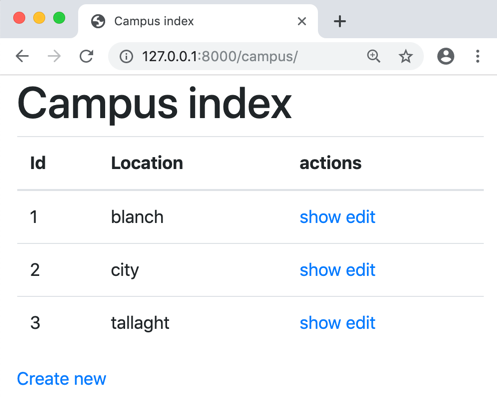
\includegraphics[width=0.75\textwidth,height=\textheight]{./tex2pdf.-2b0e1314f8bbbae5/2cc70a146aed6ecf5eeae774f90c0d07909e8e39.png}
\caption{Screenshot showing list of Campus objects.}
\end{figure}

When we create/edit a student, we now get a dropdown menu of the Campus
objects (the text in the dropdown menu is from the
\texttt{\_\_toString()} method we created for the Campus class).

\begin{figure}
\centering
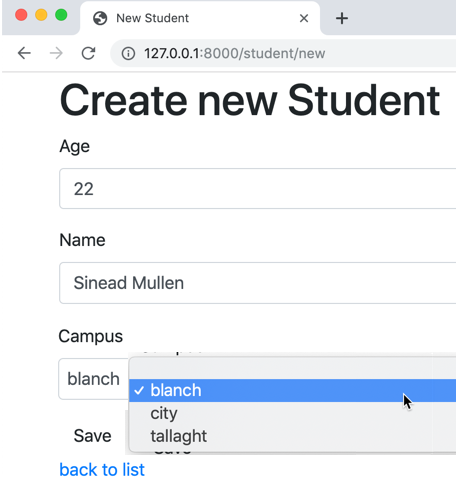
\includegraphics[width=0.75\textwidth,height=\textheight]{./tex2pdf.-2b0e1314f8bbbae5/06166ca531c57ddfbf4405cd4fecb47fcec83322.png}
\caption{Screenshot showing new Student form with Campus choice dropdown
menu}
\end{figure}

\hypertarget{customising-the-twig-templates}{%
\chapter{Customising the Twig
templates}\label{customising-the-twig-templates}}

\hypertarget{lets-add-a-new-campus-column-to-our-list-of-students}{%
\section{Let's add a new Campus column to our list of
students}\label{lets-add-a-new-campus-column-to-our-list-of-students}}

We need to edit file: \texttt{/templates/student/index.html.twig}

See Figure \ref{twig_location} for the location of this file in the
project folder structure.

\begin{figure}
\centering
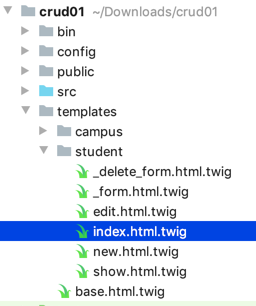
\includegraphics[width=0.5\textwidth,height=\textheight]{./tex2pdf.-2b0e1314f8bbbae5/5bc94e0457a935182217cbb4702da1ad3e17aea2.png}
\caption{Location of Twig template files. \label{twig_location}}
\end{figure}

Figure \ref{twig_before} shows the 2 places where we need to edit.

\begin{figure}
\centering
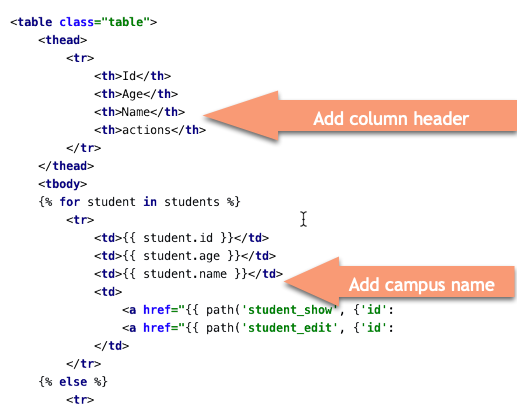
\includegraphics[width=0.75\textwidth,height=\textheight]{./tex2pdf.-2b0e1314f8bbbae5/20b62a1322e7bb7bd3888a6c41b5b13e8d2a6fda.png}
\caption{Where we will insert lines into template. \label{twig_before}}
\end{figure}

Do the following:

\begin{enumerate}
\def\labelenumi{\arabic{enumi}.}
\item
  Edit file: \texttt{/templates/student/index.html.twig}
\item
  Insert a new HTML table column header for \texttt{Campus}
\item
  Insert a new HTML table data item for \texttt{student.campus}
\end{enumerate}

Figure \ref{twig_before} shows how the file should look now - after the
lines have been inserted.

\begin{figure}
\centering
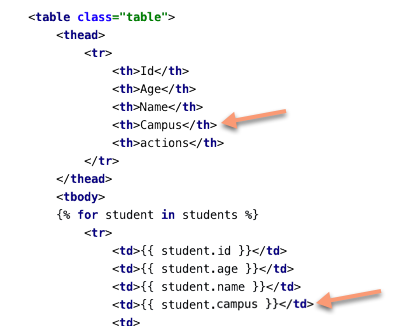
\includegraphics[width=0.75\textwidth,height=\textheight]{./tex2pdf.-2b0e1314f8bbbae5/84227cafca4ff9fdb2c37c865008a110e806146d.png}
\caption{Twig template after lines inserted. \label{twig_after}}
\end{figure}

And when we visit \texttt{/student} we should see a campus column added
to the student details - see Figure \ref{campus_column}.

\begin{figure}
\centering
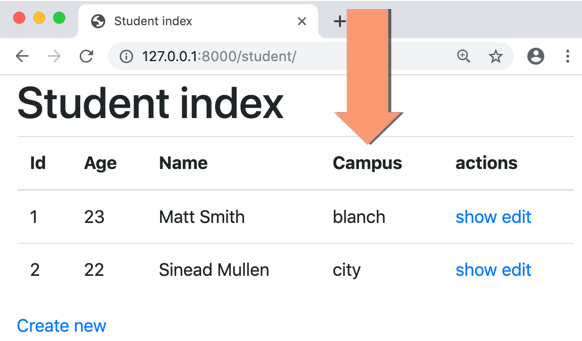
\includegraphics[width=0.75\textwidth,height=\textheight]{./tex2pdf.-2b0e1314f8bbbae5/efde51f7e3e51617cda6a160a7ed0e2815fed62f.png}
\caption{CRUD list page with extra column. \label{campus_column}}
\end{figure}

\hypertarget{turn-the-campus-name-into-a-link-to-the-related-campus-object}{%
\section{Turn the Campus name into a LINK to the related Campus
object}\label{turn-the-campus-name-into-a-link-to-the-related-campus-object}}

We can wrap an HTML hyperlink element around the campus name, to connect
our Student object to its related Campus object

Here's the edit we need to add to file:
\texttt{/templates/student/index.html.twig}

\begin{figure}
\centering
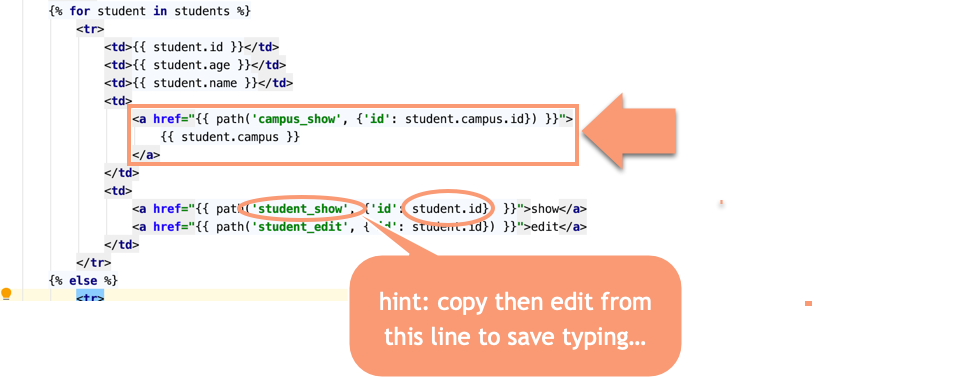
\includegraphics{./tex2pdf.-2b0e1314f8bbbae5/d15dac2f92333b46b15f191d1fa01d46678cadf6.png}
\caption{Where to edit to turn campus name into hyperlink.}
\end{figure}

When that's done, we can now click the campus and jump to the Campus
objects `show' page:

\begin{figure}
\centering
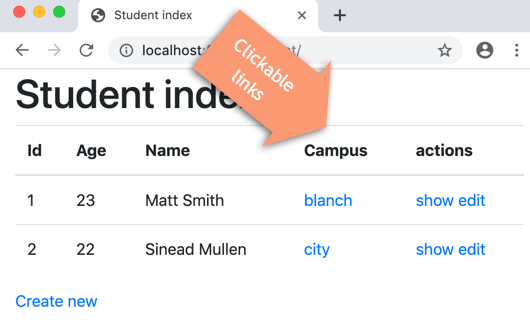
\includegraphics[width=0.75\textwidth,height=\textheight]{./tex2pdf.-2b0e1314f8bbbae5/040745e54c86e866f7782a8288615596ca63acd8.png}
\caption{Web page where campus is clickable link to Campus object.}
\end{figure}

\hypertarget{add-some-login-security}{%
\chapter{Add some login security}\label{add-some-login-security}}

\hypertarget{visit-the-user-admin-pages}{%
\section{Visit the user admin pages}\label{visit-the-user-admin-pages}}

Visit \texttt{localhost:8000/user} - you'll see our 2 users for the
system. See Figure \ref{user_index}.

\begin{verbatim}
- matt (password: smith), an **admin** user

- john (password: doe), a normal user
\end{verbatim}

\begin{figure}
\centering
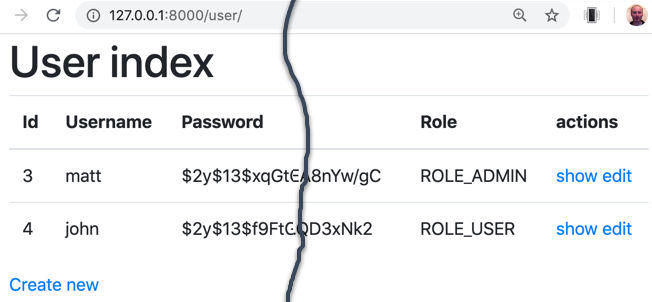
\includegraphics[width=1\textwidth,height=\textheight]{./tex2pdf.-2b0e1314f8bbbae5/802ac6fcfe8735aad07e9f15b9bdd179a6b64592.png}
\caption{Screenshot of phone make CRUD pages.\label{user_index}}
\end{figure}

These users were setup when we loaded \textbf{fixtures} (initial data)
into the database tables. These objects are created and then
\textbf{persisted} into rows in the database tables when the classes in
the \texttt{src/DataFixtures} directory are execeuted.

Since we're using several Foundry \textbf{factories}, we can create all
our test data in a few lines of code in a single class
\texttt{src/DataFixtures/AppFixtures}.

We can see the users, with their password and roles being set in the
\texttt{load(...)} method of cass class
\texttt{src/DataFixtures/AppFixtures}:

\begin{Shaded}
\begin{Highlighting}[]
    \KeywordTok{class}\NormalTok{ AppFixtures }\KeywordTok{extends}\NormalTok{ Fixture}
\NormalTok{    \{}
        \KeywordTok{public} \KeywordTok{function}\NormalTok{ load}\OtherTok{(}\NormalTok{ObjectManager }\KeywordTok{$manager}\OtherTok{)}\NormalTok{: }\KeywordTok{void}
\NormalTok{        \{}
\NormalTok{            UserFactory::createOne}\OtherTok{([}
                \StringTok{'username'}\NormalTok{ => }\StringTok{'matt'}\OtherTok{,}
                \StringTok{'password'}\NormalTok{ => }\StringTok{'smith'}\OtherTok{,}
                \StringTok{'role'}\NormalTok{ => }\StringTok{'ROLE_ADMIN'}
            \OtherTok{]);}
    
\NormalTok{            UserFactory::createOne}\OtherTok{([}
                \StringTok{'username'}\NormalTok{ => }\StringTok{'john'}\OtherTok{,}
                \StringTok{'password'}\NormalTok{ => }\StringTok{'doe'}\OtherTok{,}
                \StringTok{'role'}\NormalTok{ => }\StringTok{'ROLE_USER'}
            \OtherTok{]);}
    
\NormalTok{            MakeFactory::createOne}\OtherTok{([}\StringTok{'name'}\NormalTok{ => }\StringTok{'Apple'}\OtherTok{]);}
\NormalTok{            MakeFactory::createOne}\OtherTok{([}\StringTok{'name'}\NormalTok{ => }\StringTok{'Samsung'}\OtherTok{]);}
\NormalTok{            MakeFactory::createOne}\OtherTok{([}\StringTok{'name'}\NormalTok{ => }\StringTok{'Sony'}\OtherTok{]);}
    
\NormalTok{            PhoneFactory::createOne}\OtherTok{([}
                \StringTok{'model'}\NormalTok{ => }\StringTok{'iPhone X'}\OtherTok{,}
                \StringTok{'memory'}\NormalTok{ => }\StringTok{'128'}\OtherTok{,}
                \StringTok{'manufacturer'}\NormalTok{ => MakeFactory::find}\OtherTok{([}\StringTok{'name'}\NormalTok{ => }\StringTok{'Apple'}\OtherTok{]),}
            \OtherTok{]);}
    
\NormalTok{            PhoneFactory::createOne}\OtherTok{([}
                \StringTok{'model'}\NormalTok{ => }\StringTok{'Galaxy 21'}\OtherTok{,}
                \StringTok{'memory'}\NormalTok{ => }\StringTok{'256'}\OtherTok{,}
                \StringTok{'manufacturer'}\NormalTok{ => MakeFactory::find}\OtherTok{([}\StringTok{'name'}\NormalTok{ => }\StringTok{'Samsung'}\OtherTok{]),}
            \OtherTok{]);}
\end{Highlighting}
\end{Shaded}

\hypertarget{secure-the-user-admin-behind-a-firewall}{%
\section{Secure the user admin behind a
firewall}\label{secure-the-user-admin-behind-a-firewall}}

Let's only allow logged in ROLE\_ADMIN users to access the user CRUD
pages.

We do this by adding a requirement that a user must be logged in and
have the ROLE\_ADMIN user role. This can all be achieved by adding a
single line before the declaration of class file
\texttt{src/Controller/UserController.php}:

\begin{figure}
\centering
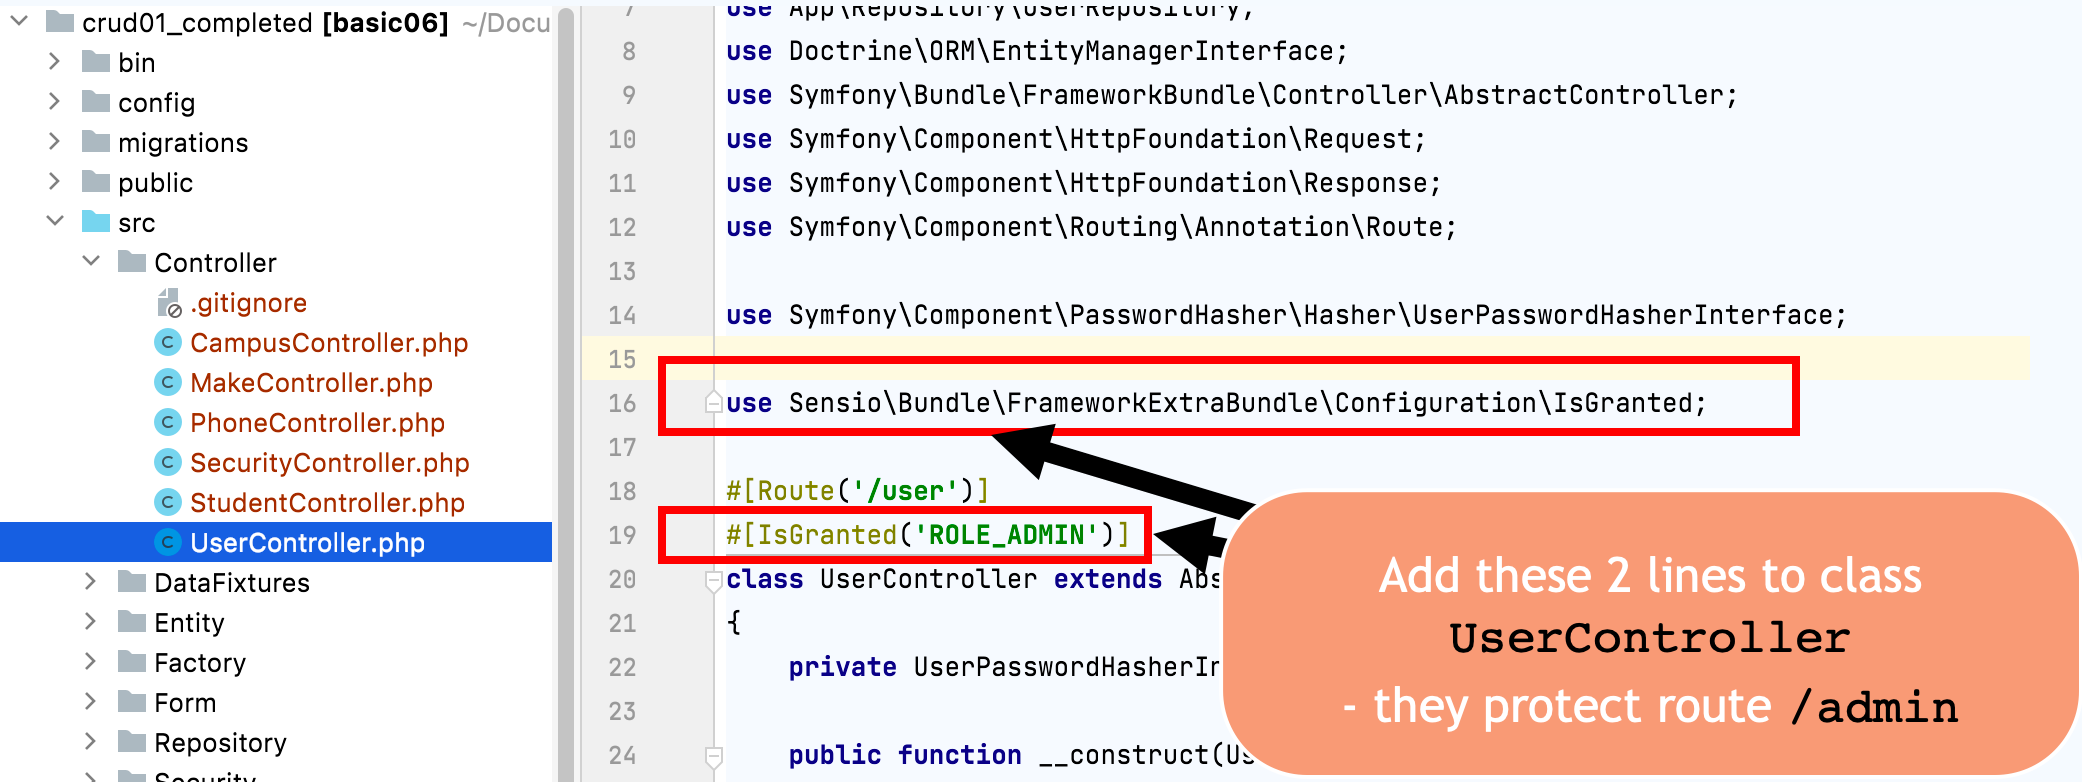
\includegraphics[width=1\textwidth,height=\textheight]{./tex2pdf.-2b0e1314f8bbbae5/a63c83bb6c49061438fa7796f13ea49e4657cae5.png}
\caption{IsGranted security requirement added to the
\texttt{UserController} class.}
\end{figure}

\hypertarget{login}{%
\section{Login}\label{login}}

If you visit \texttt{localhost:8000/user} again you'll now be asked to
login. See Figure \ref{login}.

\begin{figure}
\centering
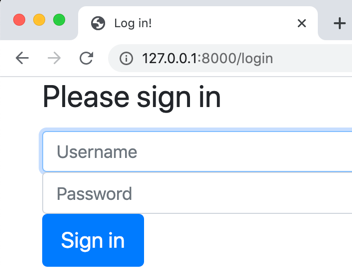
\includegraphics[width=0.5\textwidth,height=\textheight]{./tex2pdf.-2b0e1314f8bbbae5/dfbc39d266ca1d8b1fbd80ce0fe76702d4fb92f1.png}
\caption{Login form. \label{login}}
\end{figure}

If successfully logged in as an admnin user, you can now visit the user
CRUD pages. See Figure \ref{user_matt}.

\begin{figure}
\centering
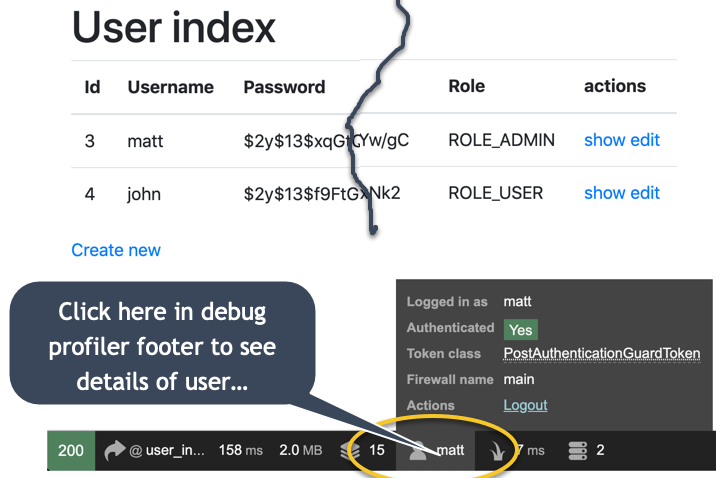
\includegraphics[width=1\textwidth,height=\textheight]{./tex2pdf.-2b0e1314f8bbbae5/84cffeb13f942d54d447415ae700cc1724cc61f3.png}
\caption{User pages logged in as \texttt{matt}. \label{user_matt}}
\end{figure}

Clicking the user in the debug profiler web page footer gives details
about the role(s) of the logged in user. See Figure
\ref{user_matt_details}.

\begin{figure}
\centering
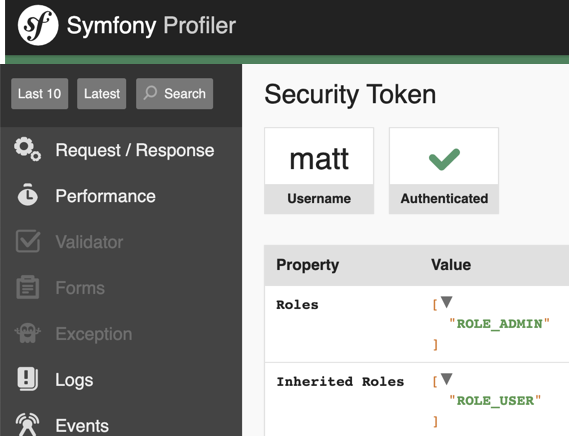
\includegraphics[width=1\textwidth,height=\textheight]{./tex2pdf.-2b0e1314f8bbbae5/2983cfab1ceb9b17b7d12ec02312c0bd2617b9da.png}
\caption{Details of logged-ion user \texttt{matt}.
\label{user_matt_details}}
\end{figure}

\part{Appendices}

\appendix

\hypertarget{software-required-for-symfony-development}{%
\chapter{\texorpdfstring{Software required for Symfony
development\label{appendix_software}}{Software required for Symfony development}}\label{software-required-for-symfony-development}}

\hypertarget{dont-confuse-different-software-tools}{%
\section{Don't confuse different software
tools}\label{dont-confuse-different-software-tools}}

Please do not confuse the following:

\begin{itemize}
\tightlist
\item
  Git and Github
\item
  PHP and PHPStorm
\end{itemize}

Here is a short description of each:

\begin{itemize}
\item
  Git: A version control system - can run locally or on networked
  computer. There are several website that support Git projects,
  including:

  \begin{itemize}
  \tightlist
  \item
    Github (perhaps the most well known)
  \item
    Gitlab
  \item
    Bitbucket
  \item
    you can also create and run your own Git web server \ldots{}
  \end{itemize}
\item
  Github: A commercial (but free for students!) cloud service for
  storing and working with projects using the Git version control system
\item
  PHP: A computer programming language, maintained by an international
  Open Source community and published at \texttt{php.net}
\item
  PHPStorm: A great (and free for student!) IDE - Interactive
  Development Environment. I.e. a really clever text editor created just
  for working with PHP projects. PHPStorm is one of the professional
  software tools offered by the \textbf{Jetbrains} company.
\end{itemize}

So in summary, Git and PHP are open source core software. Github and
PHPStorm are commercial (but free for students!) tools that support
development using Git and PHP.

\hypertarget{software-tools}{%
\section{Software tools}\label{software-tools}}

Ensure you have the following setup for developing Symfony software on
your local machine

\begin{itemize}
\tightlist
\item
  PHP 8.1.1 or later (free, open source)
\item
  Composer 2 (up-to-date with \texttt{composer\ self-update})(free, open
  source - a PHP program!)
\item
  PHPStorm (with educational free account if you're a student!) - or
  some other editor of your choice
\item
  MySQL Workbench (Community Edition free)
\item
  Git (free, open source)
\end{itemize}

See Appendix \ref{appendix_php} for checking, and if necessary,
installing PHP on your computer. See Appendix \ref{appendix_software}
for details about other software needed for working with PHP projects.

\hypertarget{test-software-by-creating-a-new-symfony-project}{%
\section{Test software by creating a new Symfony
project}\label{test-software-by-creating-a-new-symfony-project}}

Test your software by using PHP and Composer to create a new Symfony 4
project. We'll follow the steps at the
\href{https://symfony.com/doc/current/setup.html}{Symfony setup} web
page.

Follow the steps in Appendix \ref{appendix_sf_basic}.

\hypertarget{php-windows-setup}{%
\chapter{\texorpdfstring{PHP Windows
setup\label{appendix_php}}{PHP Windows setup}}\label{php-windows-setup}}

\hypertarget{check-if-you-have-php-installed-and-working}{%
\section{Check if you have PHP installed and
working}\label{check-if-you-have-php-installed-and-working}}

You need PHP version 8.1.1 or later.

Check your PHP version at the command line with:

\begin{Shaded}
\begin{Highlighting}[]
   \OperatorTok{>} \ExtensionTok{php}\NormalTok{ -v}
   \ExtensionTok{PHP}\NormalTok{ 8.1.1 (cli) }\KeywordTok{(}\ExtensionTok{built}\NormalTok{: Dec 15 2021 09:54:28}\KeywordTok{)} \KeywordTok{(}\ExtensionTok{NTS}\KeywordTok{)}
   \ExtensionTok{Copyright}\NormalTok{ (c) }\ExtensionTok{The}\NormalTok{ PHP Group}
   \ExtensionTok{Zend}\NormalTok{ Engine v4.1.1, Copyright (c) }\ExtensionTok{Zend}\NormalTok{ Technologies}
       \ExtensionTok{with}\NormalTok{ Zend OPcache v8.1.1, Copyright (c), }\ExtensionTok{by}\NormalTok{ Zend Technologies}
\end{Highlighting}
\end{Shaded}

If your version is older than 8.1.1, or you get an error about command
not understood, then complete the steps below.

\hypertarget{download-the-latest-version-of-php}{%
\subsection{Download the latest version of
PHP}\label{download-the-latest-version-of-php}}

Get the latest (8.1.1 at the time of writing) PHP Windows ZIP from:

\begin{itemize}
\tightlist
\item
  \href{http://php.net/downloads.php}{php.net} click the \textbf{Windows
  Downloads} link
\end{itemize}

NOTE: If installing on Windows ensure you are \textbf{displaying file
extensions}, e.g.~so you see \texttt{php.exe} and \texttt{php.ini} not
just \texttt{php} - Don't relyon Windows to show the right icon while
\emph{hiding the full filename}\ldots{}

Figure \ref{windows_zip} shows a screenshot of the \texttt{php.net}
general and Windows downloads page. The \texttt{ZIP} file to download
(containing \texttt{php.exe} \ldots{} don't download the source code
version unless you want to build the file from code \ldots{}):

\begin{figure}
\centering
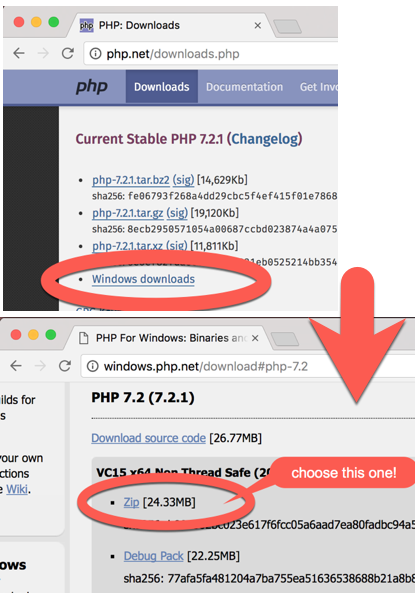
\includegraphics{./tex2pdf.-2b0e1314f8bbbae5/54ea2bd7518c42f7055083e08168bc8498c402b7.png}
\caption{PHP.net / Windows ZIP download pages. \label{windows_zip}}
\end{figure}

Do the following:

\begin{itemize}
\item
  unzip the PHP folder into: \texttt{C:\textbackslash{}php}
\item
  so you should now have a file \texttt{php.exe} inside
  \texttt{C:\textbackslash{}php}, along with lots of other files
\item
  make a copy the file
  \texttt{C:\textbackslash{}php\textbackslash{}php.ini-development},
  naming the copy \texttt{C:\textbackslash{}php\textbackslash{}php.ini}
\end{itemize}

\hypertarget{add-the-path-to-php.exe-to-your-system-environment-variables}{%
\section{\texorpdfstring{Add the \textbf{path} to \texttt{php.exe} to
your System environment
variables}{Add the path to php.exe to your System environment variables}}\label{add-the-path-to-php.exe-to-your-system-environment-variables}}

Whenever you type a command at the CLI (Command Line Interface) Windows
searches through all the directories in its \texttt{path} environment
variable. In order to use PHP at the CLI we need to add
\texttt{c:\textbackslash{}php} to the \texttt{path} environment variable
so the \texttt{php.exe} executable can be found.

Via the System Properties editor, open your Windows Environment
Variables editor. The \textbf{system} environment variables are in the
lower half of the Environment Variables editor. If there is already a
system variable named \texttt{Path}, then select it and click the
\textbf{Edit} button. If none exists, then click the \textbf{New}
button, naming the new variable \textbf{path}. Add a new value to the
\textbf{path} variable with the value \texttt{c:\textbackslash{}php}.
Then click all the \textbf{Okay} buttons needed to close all these
windows.

Now open a windows \textbf{Cmd} window and try the \texttt{php\ -v} -
hopefully you'll see confirmation that your system now has PHP installed
and in the \textbf{path} for CLI commands.

Figure \ref{env2} shows a screenshot of the Windows system and
environment variables editor.

\begin{figure}
\centering
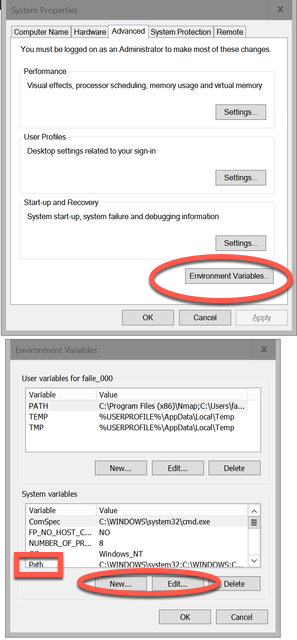
\includegraphics{./tex2pdf.-2b0e1314f8bbbae5/eb1ab9d21c784b824e4103ff64f0448e7b0e6122.png}
\caption{The Windows Environment Variables editor. \label{env2}}
\end{figure}

\hypertarget{check-your-php.ini-file}{%
\section{\texorpdfstring{Check your \texttt{php.ini}
file}{Check your php.ini file}}\label{check-your-php.ini-file}}

Open a new terminal CLI window (so new settings are loaded) and run
\texttt{php\ -\/-ini} to confirm the location of the \texttt{php.ini}
file that you've just created. Note the following for a Mac - for
Windows it should (hopefully) tell you it found the ini file in
\texttt{c:\textbackslash{}php\textbackslash{}php.ini}:

\begin{Shaded}
\begin{Highlighting}[]
\NormalTok{    $ }\ExtensionTok{php}\NormalTok{ --ini}
    \ExtensionTok{Configuration}\NormalTok{ File (php.ini) }\ExtensionTok{Path}\NormalTok{: /Applications/MAMP/bin/php/php7.1.8/conf}
    \ExtensionTok{Loaded}\NormalTok{ Configuration File:         /Applications/MAMP/bin/php/php7.1.8/conf/php.ini}
    \ExtensionTok{Scan}\NormalTok{ for additional .ini files in: (none)}
    \ExtensionTok{Additional}\NormalTok{ .ini files parsed:      (none)}
\end{Highlighting}
\end{Shaded}

\hypertarget{php-info-sql-driver-test}{%
\section{PHP Info \& SQL driver test}\label{php-info-sql-driver-test}}

For database work we need to enable the PDO\footnote{PDO = PHP Database
  Objects, the modern library for managing PHP program communications
  with databases. Avoid using old libries like \texttt{mysql} (security
  issues) and even \texttt{mysqli} (just for MySQL). PDO offers an
  object-oriented, standardized way to communicate with many different
  database systems. So a project could change the databse management
  system (e.g.~from Oracle to MySQL to SQLite), and only the database
  connetion optins need to change - all other PDO code will work with
  the new database system!} options for MySQL and SQLite (see later
database exercises for how to do this)

Although PHP may have been installed, and its SQL drivers too, they may
have not been enabled. For this module we'll be using the SQLite and
MySQL drivers for PHP -- to talk to databases. The function
\texttt{phpinfo()} is very useful since it displays many of the settings
of the PHP installation on your computer / website.

\begin{enumerate}
\def\labelenumi{\arabic{enumi}.}
\item
  In the current (or a temporary) direcotry, create file
  \texttt{info.php} containing just the following 2 lines of code:

\begin{Shaded}
\begin{Highlighting}[]
\NormalTok{    <}\OtherTok{?}\NormalTok{php}
    \KeywordTok{print} \FunctionTok{phpinfo}\OtherTok{();}
\end{Highlighting}
\end{Shaded}
\item
  At the CLI run the built-in PHP web server to serve this page, and
  visit: \texttt{localhost:8000/info.php} in your web browser

\begin{Shaded}
\begin{Highlighting}[]
    \ExtensionTok{php}\NormalTok{ -S localhost:8000}
\end{Highlighting}
\end{Shaded}
\end{enumerate}

In the PDO section of the web page (\texttt{CTL-F} and search for
\texttt{pdo} \ldots{}) we are looking for \textbf{mysql} and
\textbf{sqlite}. If you see these then great!

Figure \ref{info} shows a screenshot the Windows system and environment
variables editor.

\begin{figure}
\centering
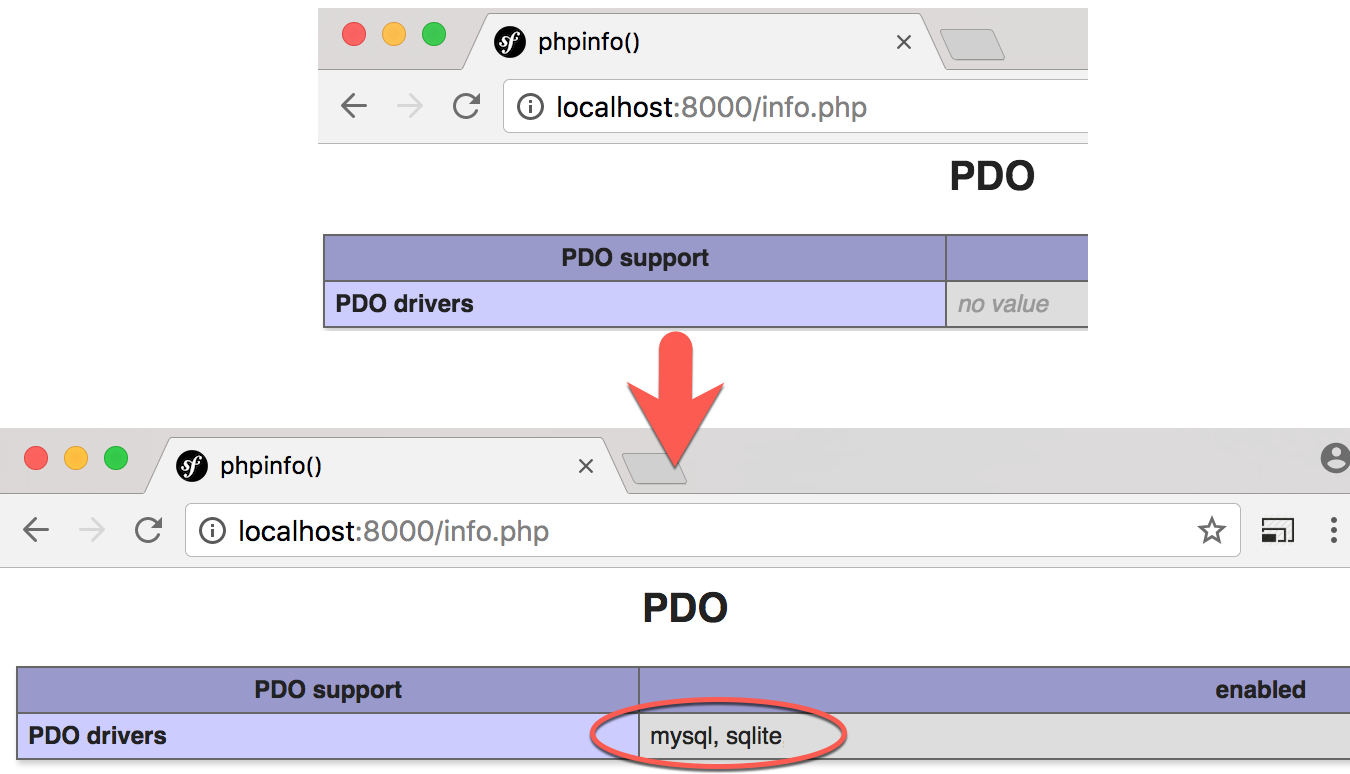
\includegraphics{./tex2pdf.-2b0e1314f8bbbae5/23f96bdd9781fe840d266ef37cf21f53375d2ee1.png}
\caption{The PDO section of the \texttt{phpinfo()} information page.
\label{info}}
\end{figure}

But, if you see ``no value'' under the PDO drivers section, then we'll
need to edit file \texttt{c:\textbackslash{}php\textbackslash{}php.ini}:

\begin{enumerate}
\def\labelenumi{\arabic{enumi}.}
\tightlist
\item
  In a text editor open file
  \texttt{c:\textbackslash{}php\textbackslash{}php.ini} and locate the
  ``Dynamic Extensions'' section in this file (e.g.~use the editor
  Search feature - or you could just search for \texttt{pdo})
\end{enumerate}

\begin{figure}
\centering
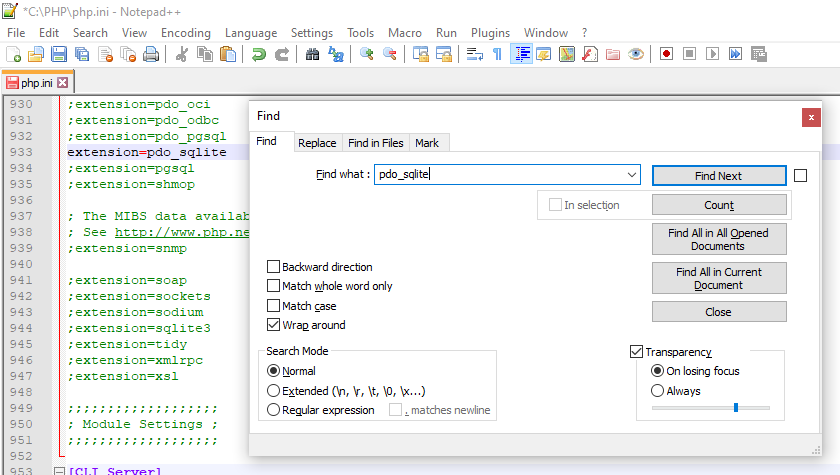
\includegraphics{./tex2pdf.-2b0e1314f8bbbae5/1d5fcbd6fa656ccd94d4e29a62daf0a1df5dae28.png}
\caption{SQLite being enabled in php.ini in the Notepad++ editor.}
\end{figure}

\begin{enumerate}
\def\labelenumi{\arabic{enumi}.}
\setcounter{enumi}{1}
\item
  Now remove the semi-colon \texttt{;} comment character at the
  beginning of the lines for the SQLite and MySQL DLLs to enable them as
  shown here:

\begin{Shaded}
\begin{Highlighting}[]
\NormalTok{    ;;;;;;;;;;;;;;;;;;;;;;}
\NormalTok{    ; }\ExtensionTok{Dynamic}\NormalTok{ Extensions }\KeywordTok{;}
\NormalTok{    ;;;;;;;;;;;;;;;;;;;;;;}

    \ExtensionTok{..}\NormalTok{ other lines here ...}
    \VariableTok{extension=}\NormalTok{php_pdo_mysql }\OperatorTok{<<<<<<<<<<} \ExtensionTok{here}\NormalTok{ is the PDO MYSQL driver line}
\NormalTok{    ;}\VariableTok{extension=}\NormalTok{php_pdo_oci}
\NormalTok{    ;}\VariableTok{extension=}\NormalTok{php_pdo_odbc}
\NormalTok{    ;}\VariableTok{extension=}\NormalTok{php_pdo_pgsql}
    \VariableTok{extension=}\NormalTok{php_pdo_sqlite }\OperatorTok{<<<<<<<<  here} \ExtensionTok{is}\NormalTok{ the PDO SQLITE driver line}
\end{Highlighting}
\end{Shaded}
\item
  Save the file. Close your Command Prompt, and re-open it (to ensure
  new settings are used).

  -- Run the webserver again and visit: \texttt{localhost:8000/info.php}
  to check the PDO drivers.
\end{enumerate}

NOTE: Knowing how to view \texttt{phpinfo()} is very handy when checking
server features.

\hypertarget{the-composer-andd-symfony-command-line-tools}{%
\chapter{\texorpdfstring{The Composer andd Symfony command line
tools\label{cli_tools}}{The Composer andd Symfony command line tools}}\label{the-composer-andd-symfony-command-line-tools}}

\hypertarget{composer}{%
\section{Composer}\label{composer}}

Composer is a \textbf{fantastic} PHP tool for managing project
dependencies (the libraries and class packages used by OO PHP projects).

\begin{enumerate}
\def\labelenumi{\arabic{enumi}.}
\item
  ensure that Composer is up to date by running:

\begin{Shaded}
\begin{Highlighting}[]
    \ExtensionTok{composer}\NormalTok{ self-update}
\end{Highlighting}
\end{Shaded}
\item
  enable the PDO options for MySQL and SQLite (see Appendix
  \ref{appendix_php} for how to do this by editing ther
  \texttt{c:\textbackslash{}php\textbackslash{}php.ini} file \ldots{})
\end{enumerate}

The Composer tool is actually a \textbf{PHAR} (PHP Archive) - i.e.~a PHP
application packaged into a single file. So ensure you have PHP
installed and in your environment \textbf{path} before attempting to
install or use Composer.

Ensure you have (or install) an up-to-date version of the Composer PHP
package manager.

\begin{Shaded}
\begin{Highlighting}[]
    \ExtensionTok{composer}\NormalTok{ self-update}
\end{Highlighting}
\end{Shaded}

\hypertarget{windows-composer-install}{%
\subsection{Windows Composer install}\label{windows-composer-install}}

Get the latest version of Composer from

\begin{itemize}
\item
  \href{https://getcomposer.org/}{getcomposer.org}
\item
  run the provided \textbf{Composer-Setup.exe} installer (just accept
  all the default options - do NOT tick the developer mode)

  -- \url{https://getcomposer.org/doc/00-intro.md\#installation-windows}
  \#\# The Composer PHP library tool
\end{itemize}

The Composer tool is actually a \textbf{PHAR} (PHP Archive) - i.e.~a PHP
application packaged into a single file. So ensure you have PHP
installed and in your environment \textbf{path} before attempting to
install or use Composer.

Ensure you have (or install) an up-to-date version of the Composer PHP
package manager.

\begin{Shaded}
\begin{Highlighting}[]
    \ExtensionTok{composer}\NormalTok{ self-update}
\end{Highlighting}
\end{Shaded}

\hypertarget{windows-composer-install-1}{%
\subsection{Windows Composer install}\label{windows-composer-install-1}}

Get the latest version of Composer from

\begin{itemize}
\item
  \href{https://getcomposer.org/}{getcomposer.org}
\item
  run the provided \textbf{Composer-Setup.exe} installer (just accept
  all the default options - do NOT tick the developer mode)

  -- \url{https://getcomposer.org/doc/00-intro.md\#installation-windows}
\end{itemize}

\hypertarget{symfony-command-line-tool}{%
\section{Symfony command line tool}\label{symfony-command-line-tool}}

Install this from:

\begin{itemize}
\tightlist
\item
  \url{https://symfony.com/download}
\end{itemize}

at the time of writing the version of this CLI was:

\begin{Shaded}
\begin{Highlighting}[]
\NormalTok{  $ }\ExtensionTok{symfony}
  \ExtensionTok{Symfony}\NormalTok{ CLI version 5.2.1 (c) }\ExtensionTok{2017-2022}\NormalTok{ Symfony SAS (2022-01-22T17:14:23Z - stable)}
\end{Highlighting}
\end{Shaded}

\hypertarget{software-tools-1}{%
\chapter{\texorpdfstring{Software
tools\label{appendix_software_setup}}{Software tools}}\label{software-tools-1}}

NOTE: All the following should already available on the college
computers.

\hypertarget{phpstorm-editor}{%
\section{PHPStorm editor}\label{phpstorm-editor}}

Ensure you have your free education Jetbrains licence from:

\begin{itemize}
\tightlist
\item
  \href{https://www.jetbrains.com/shop/eform/students}{Students form:
  https://www.jetbrains.com/shop/eform/students} (ensure you use your
  ITB student email address)
\end{itemize}

Downdload and install PHPStorm from:

\begin{itemize}
\tightlist
\item
  \url{https://www.jetbrains.com/phpstorm/download/}
\end{itemize}

To save lots of typing, try to install the following useful PHPStorm
plugins:

\begin{itemize}
\tightlist
\item
  Twig
\item
  Symfony
\item
  Annotations
\end{itemize}

\hypertarget{mysql-workbench}{%
\section{MySQL Workbench}\label{mysql-workbench}}

While you can work with SQLite and other database management systems,
many ITB modules use MySQLWorkbench for database work, and it's fine, so
that's what we'll use (and, of course, it is already installed on the
ITB windows computers \ldots{})

Download and install MySQL Workbench from:

\begin{itemize}
\tightlist
\item
  \url{https://dev.mysql.com/downloads/workbench/}
\end{itemize}

\hypertarget{git}{%
\section{Git}\label{git}}

Git is a fantastic (and free!) DVCS - Distributed Version Control
System. It has free installers for Windows, Mac, Linus etc.

Check is Git in installed on your computer by typing \texttt{git} at the
CLI terminal:

\begin{Shaded}
\begin{Highlighting}[]
    \OperatorTok{>} \FunctionTok{git}
    \ExtensionTok{usage}\NormalTok{: git [--version] [--help] [-C }\OperatorTok{<}\NormalTok{path}\OperatorTok{>}\NormalTok{] [-c name=value]}
\NormalTok{               [}\ExtensionTok{--exec-path}\NormalTok{[=}\OperatorTok{<}\NormalTok{path}\OperatorTok{>}\NormalTok{]] [--html-path] [--man-path] [--info-path]}
\NormalTok{               [}\ExtensionTok{-p} \KeywordTok{|} \ExtensionTok{--paginate} \KeywordTok{|} \ExtensionTok{--no-pager}\NormalTok{] [--no-replace-objects] [--bare]}
\NormalTok{               [}\ExtensionTok{--git-dir}\NormalTok{=}\OperatorTok{<}\NormalTok{path}\OperatorTok{>}\NormalTok{] [--work-tree=}\OperatorTok{<}\NormalTok{path}\OperatorTok{>}\NormalTok{] [--namespace=}\OperatorTok{<}\NormalTok{name}\OperatorTok{>}\NormalTok{]}
               \OperatorTok{<}\BuiltInTok{command}\OperatorTok{>}\NormalTok{ [}\OperatorTok{<}\NormalTok{args}\OperatorTok{>}\NormalTok{]}

    \ExtensionTok{These}\NormalTok{ are common Git commands used in various situations:}

    \ExtensionTok{start}\NormalTok{ a working area (see also: git help tutorial)}
       \ExtensionTok{clone}\NormalTok{      Clone a repository into a new directory}
       \ExtensionTok{init}\NormalTok{       Create an empty Git repository or reinitialize an existing one}

    \ExtensionTok{...}

    \ExtensionTok{collaborate}\NormalTok{ (see also: git help workflows)}
       \ExtensionTok{fetch}\NormalTok{      Download objects and refs from another repository}
       \ExtensionTok{pull}\NormalTok{       Fetch from and integrate with another repository or a local branch}
       \ExtensionTok{push}\NormalTok{       Update remote refs along with associated objects}

    \StringTok{'git help -a'} \ExtensionTok{and} \StringTok{'git help -g'}\NormalTok{ list available subcommands and some}
    \ExtensionTok{concept}\NormalTok{ guides. See }\StringTok{'git help <command>'}\NormalTok{ or }\StringTok{'git help <concept>'}
    \ExtensionTok{to}\NormalTok{ read about a specific subcommand or concept.}

    \OperatorTok{>}
\end{Highlighting}
\end{Shaded}

If you don't see a list of \textbf{Git} commands like the above, then
you need to install Git on your computer.

\hypertarget{git-windows-installation}{%
\section{Git Windows installation}\label{git-windows-installation}}

Visit this page to run the Windows Git installer.

\begin{itemize}
\tightlist
\item
  \url{https://git-scm.com/downloads}
\end{itemize}

NOTE: Do \textbf{not} use a GUI-git client. Do all your Git work at the
command line. It's the best way to learn, and it means you can work with
Git on other computers, for remote terminal sessions (e.g.~to work on
remote web servers) and so on.

\end{document}
